\appendix

\section{Experimental Setup of \S\ref{subsec:significance_of_prefix_homogeneity}}
\subsection{Two Large Prefixes - Heterogeneity}
\label{subsec:two_large_prefixes_heterogeneity}
Figure~\ref{fig:two_fam_vis} shows the visualization of the experiment corresponding to takeaway 1 of \S\ref{sec:motivation}. We have a total of 500 requests, each using one of the prefixes $A$ or $B$. These prefixes are 10K tokens long, and each query has a unique 20 token-long suffix. $f \in [0,1]$ denotes the fraction of requests using prefix $A$. When $f$ is either 0 or 1, the batch is homogeneous; otherwise, two prefix groups coexist.

\begin{figure}[b]
\vspace{-10pt}
\centering
\begin{minipage}{0.80\columnwidth}
    \centering
    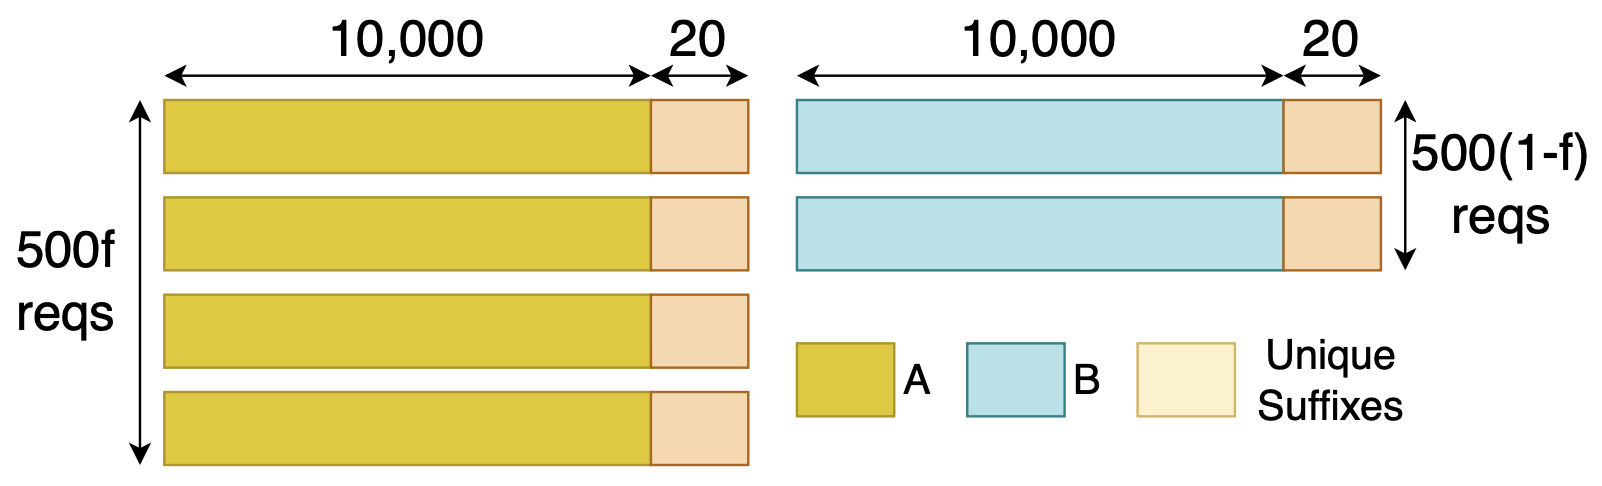
\includegraphics[width=\linewidth]{illustration_images/two_family_experiment.png}
    \caption{Two Large Prefixes}
    \label{fig:two_fam_vis}
\end{minipage}
\vspace{-15pt}
\end{figure}

\subsection{Fractional Sharing}
\label{subsec:fractional_sharing}
Figure~\ref{fig:frac_share_vis} shows the visualization of the experiment corresponding to takeaway 2 of \S\ref{sec:motivation}. We have a total of 100 requests, each with a length of 2K tokens. Each request shares a common prefix of length $2K \times f$ tokens, where $f \in [0, 1]$, with the remaining $2K \times (1-f)$ unique.

\begin{figure}[t]
\centering
\begin{minipage}{0.70\columnwidth}
    \centering
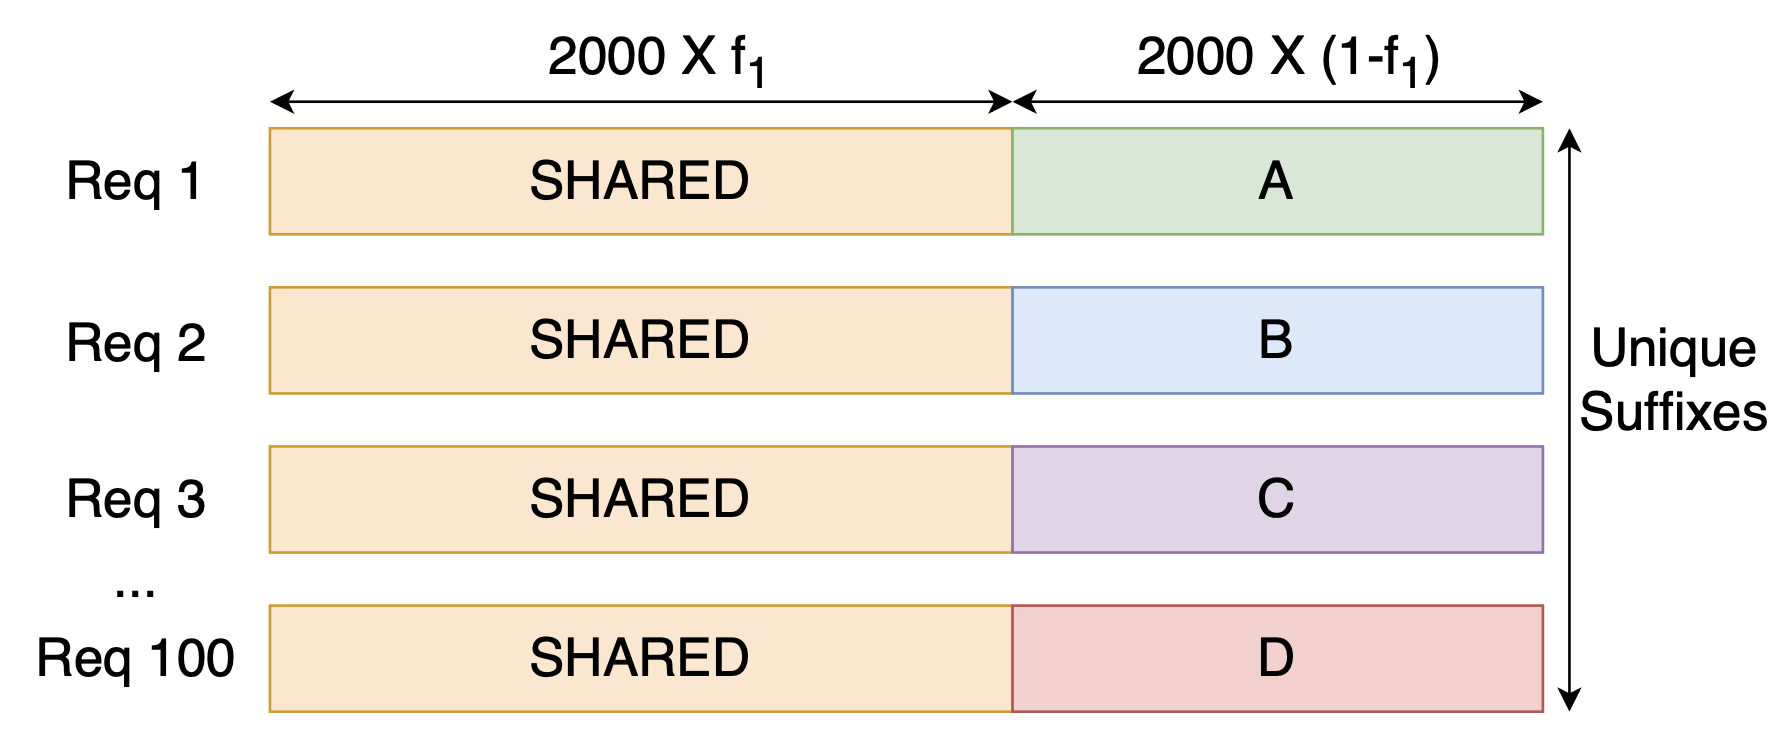
\includegraphics[width=\columnwidth]{illustration_images/fractional_sharing_experiment.png}
\caption{Fractional Sharing}
\label{fig:frac_share_vis}
\end{minipage}
\vspace{-10pt}
\end{figure}

\subsection{Radix Tree Sharing Patterns}
\label{subsec:radix_tree_sharing_patterns}
Figure~\ref{fig:sharing_configurations} shows the visualization corresponding to takeaway 4 in \S\ref{sec:motivation}. We consider four different radix tree sharing patterns. The sequence length in each case is fixed at $4L$.
(i) In Figure~\ref{fig:vis_complete_sharing}, the entire $4L$ prefix is shared across all requests.
(ii) In Figure~\ref{fig:2_levels}, the tree has two levels. The first level, of length $L$, is shared by all requests, while the second level consists of two branches, each of length $3L$.
(iii) In Figure~\ref{fig:3_levels}, the tree has three levels with lengths $L$, $L$, and $2L$, and with 1, 2, and 4 branches at each level, respectively.
(iv) In Figure~\ref{fig:4_levels}, the tree has four levels, each of length $L$, with 1, 2, 4, and 8 branches at successive levels.

\begin{figure}[t]
    \centering
    \captionsetup[subfigure]{labelformat=simple}
    \renewcommand\thesubfigure{(\alph{subfigure})}
    \begin{subfigure}{0.12\columnwidth}
        \centering
        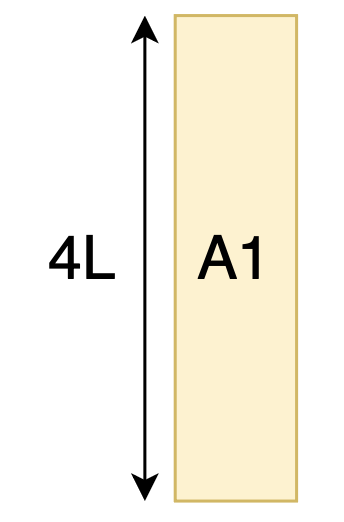
\includegraphics[width=\linewidth]{illustration_images/vis_complete_sharing.png}
        \caption{1-level}
        \label{fig:vis_complete_sharing}
    \end{subfigure}
    \hfill
    \begin{subfigure}{0.17\columnwidth}
        \centering
        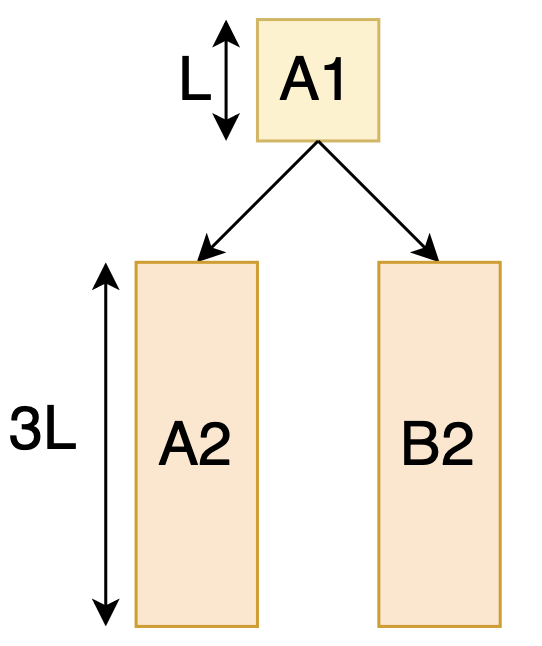
\includegraphics[width=\linewidth]{illustration_images/vis_2_levels.png}
        \caption{2 levels}
        \label{fig:2_levels}
    \end{subfigure}
    \hfill
    \begin{subfigure}{0.27\columnwidth}
        \centering
        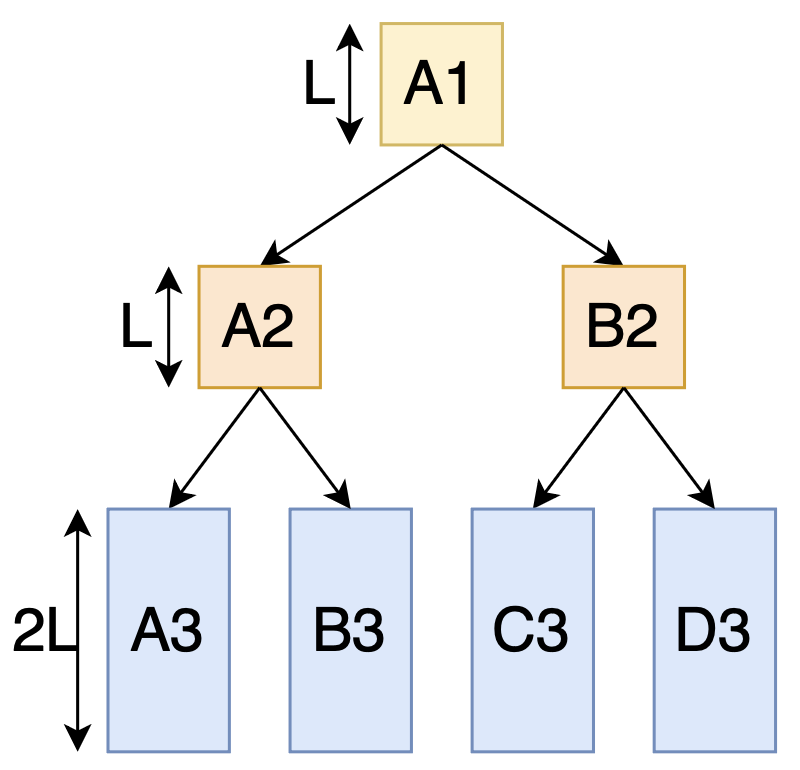
\includegraphics[width=\linewidth]{illustration_images/vis_3_levels.png}
        \caption{3 levels}
        \label{fig:3_levels}
    \end{subfigure}
    \hfill
    \begin{subfigure}{0.40\columnwidth}
        \centering
        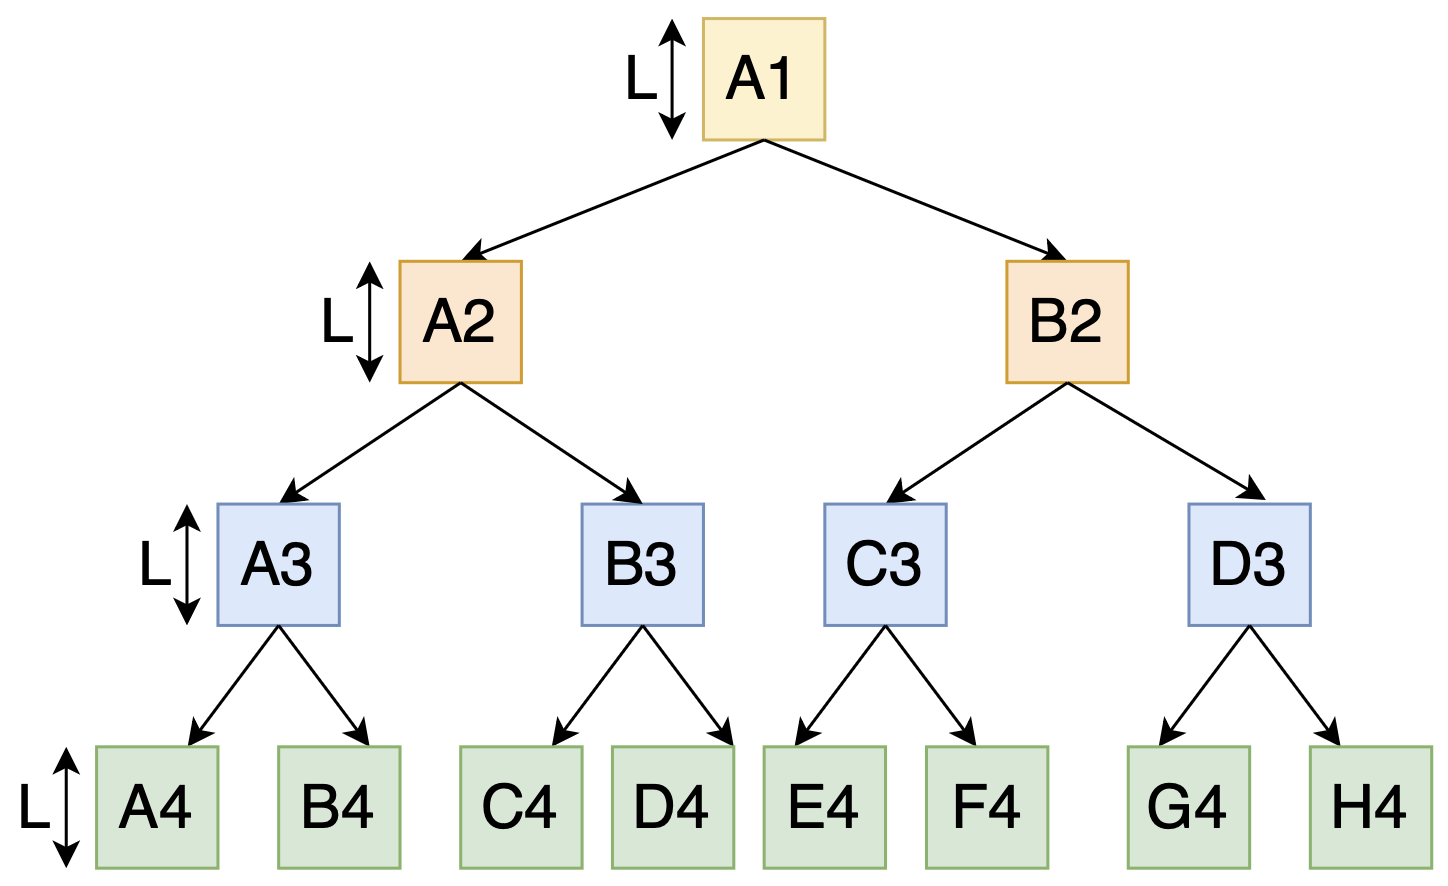
\includegraphics[width=\linewidth]{illustration_images/vis_4_levels.png}
        \caption{4 levels}
        \label{fig:4_levels}
    \end{subfigure}
    \caption{Radix Tree Sharing Levels}
    \label{fig:sharing_configurations}
    \vspace{-10pt}
\end{figure}

\section{Additional Results from \S\ref{subsec:significance_of_prefix_homogeneity}}
\label{sec:additional_results_section_3}
Below, we present a set of experiments to strengthen our observations from \S\ref{subsec:significance_of_prefix_homogeneity} regarding prefix homogeneity.

\subsection{Effect of Total KV Cache Size}
\label{subsec:cache_working_set_theory}
Figure~\ref{fig:qwen_tp_kvcache} illustrates vLLM's FCFS throughput alongside the total KV cache memory footprint for prefix tokens in the Qwen 0.5B model, evaluated across varying prefix lengths and numbers of prefix groups. As expected, throughput decreases as the prefix sequence length increases. A more pronounced drop is observed when the number of prefix groups increases from 1 to 2, which can be attributed to a loss of locality. Beyond this point, however, throughput remains relatively stable. This suggests that increasing the number of prefix groups further does not significantly degrade temporal or spatial locality, indicating that most of the locality loss occurs in the transition from a single group to multiple groups. Moreover, this drop from 1 to 2 prefix groups is observable only for larger shared prefix lengths where temporal and spatial locality benefits kick in.

Another question to ask if the high throughput values are correlated with the entire KV cache working set fitting into one of the cache levels. L1 cache size is typically in KBs, which is too small even for tens of tokens. Therefore, we focus on the L2 cache, which is 96 MB in size for the GPU on which these experiments were run. In the top-left region of the heatmap, the entire KV cache fits within this size. However, no clear throughput degradation is observed once this threshold is exceeded. This indicates that effective spatial and temporal locality depend more on whether the subset of KV blocks actively accessed by batched requests at a given time (i.e. the dynamic working set) fits in the L2 cache. It is intuitive that this dynamic working set is smaller in size for prefix-homogeneous batches which explains the higher throughput gains achieved for such batches. Moreover, even for such a small model, the model weights are already large enough to prevent the entire KV cache to reside in L2. Therefore, performance gains due to prefix homogeneity primarily stem from a smaller dynamic working set of the KV cache.

\begin{figure}[t]
\captionsetup[subfigure]{labelformat=simple}
    \renewcommand\thesubfigure{(\alph{subfigure})}
\centering
\begin{subfigure}{0.49\columnwidth}
    \centering
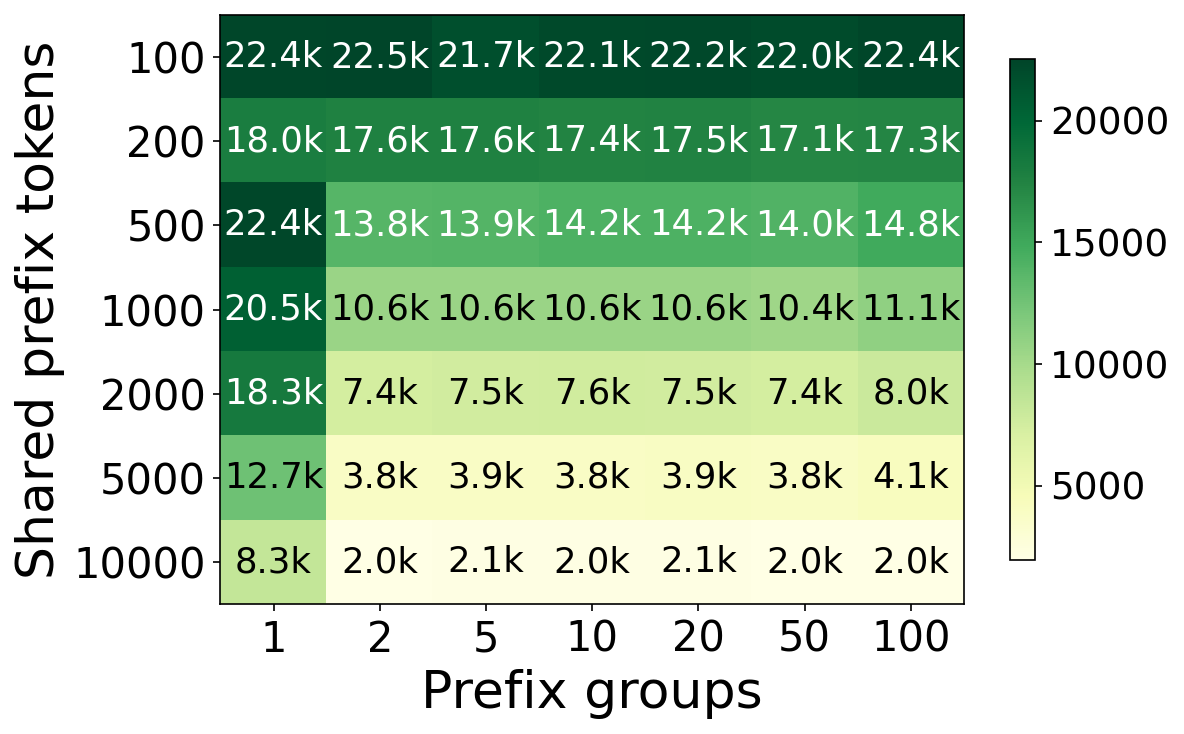
\includegraphics[width=\linewidth]{results/qwen_working_set_theory_plots/vllm_heatmap_throughput.png}
\caption{Throughput}
\label{fig:tp_qwen}
\end{subfigure}
\hfill
\begin{subfigure}{0.49\columnwidth}
    \centering
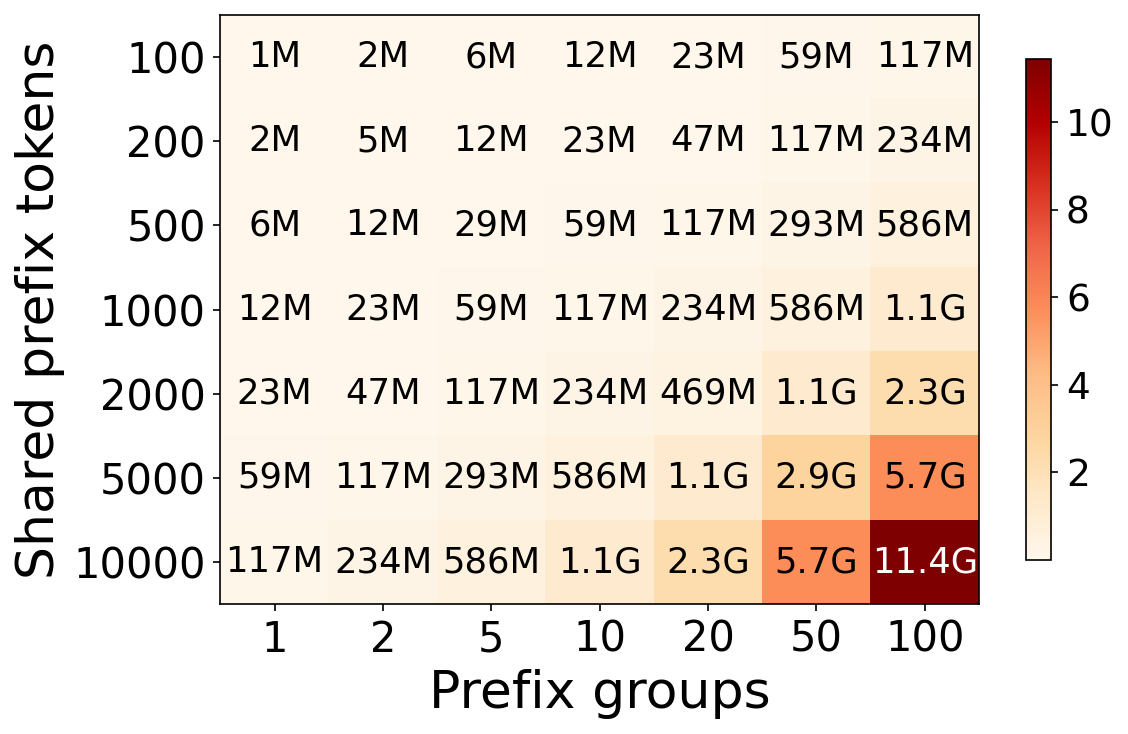
\includegraphics[width=\linewidth]{results/qwen_working_set_theory_plots/vllm_heatmap_kvcache.png}
\caption{KV Cache Memory}
\label{fig:kvcache}
\end{subfigure}
\caption{Throughput and KV Cache Size}
\label{fig:qwen_tp_kvcache}
\vspace{-10pt}
\end{figure}

\begin{figure}[t]
\captionsetup[subfigure]{labelformat=simple}
    \renewcommand\thesubfigure{(\alph{subfigure})}
\centering
\begin{subfigure}{0.49\columnwidth}
    \centering
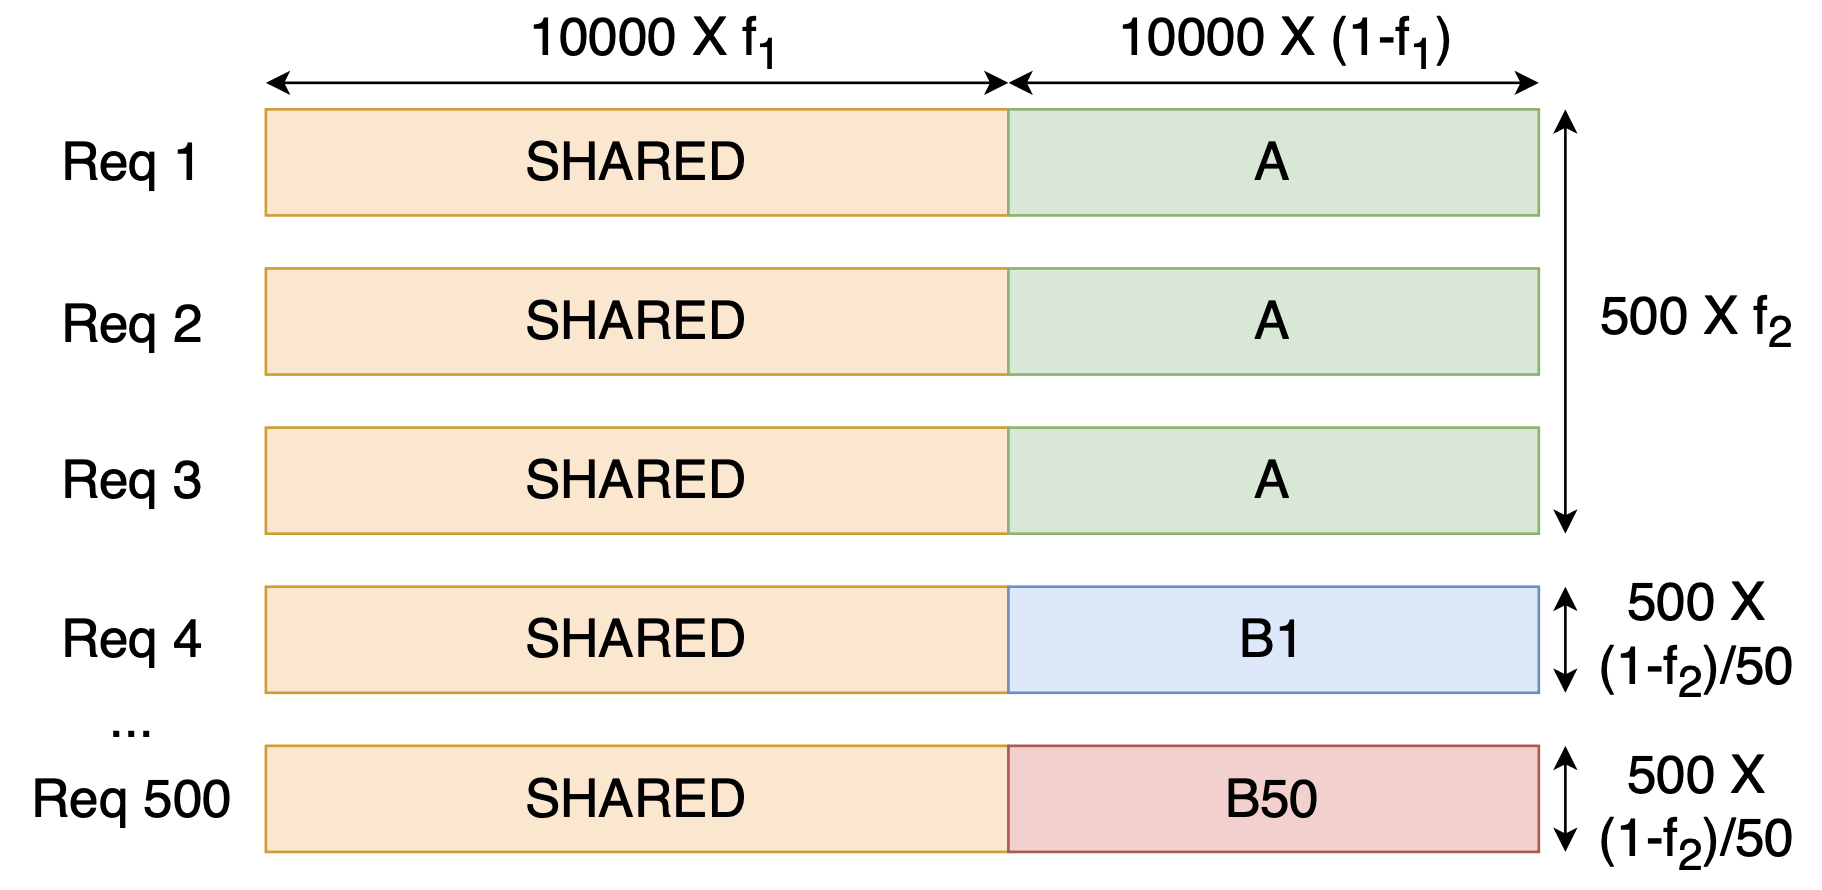
\includegraphics[width=\columnwidth]{illustration_images/tiered_prefix_sharing.png}
\caption{Visualization}
\label{fig:vis_tiered_prefix_sharing}
\end{subfigure}
\hfill
\begin{subfigure}{0.49\columnwidth}
   \centering
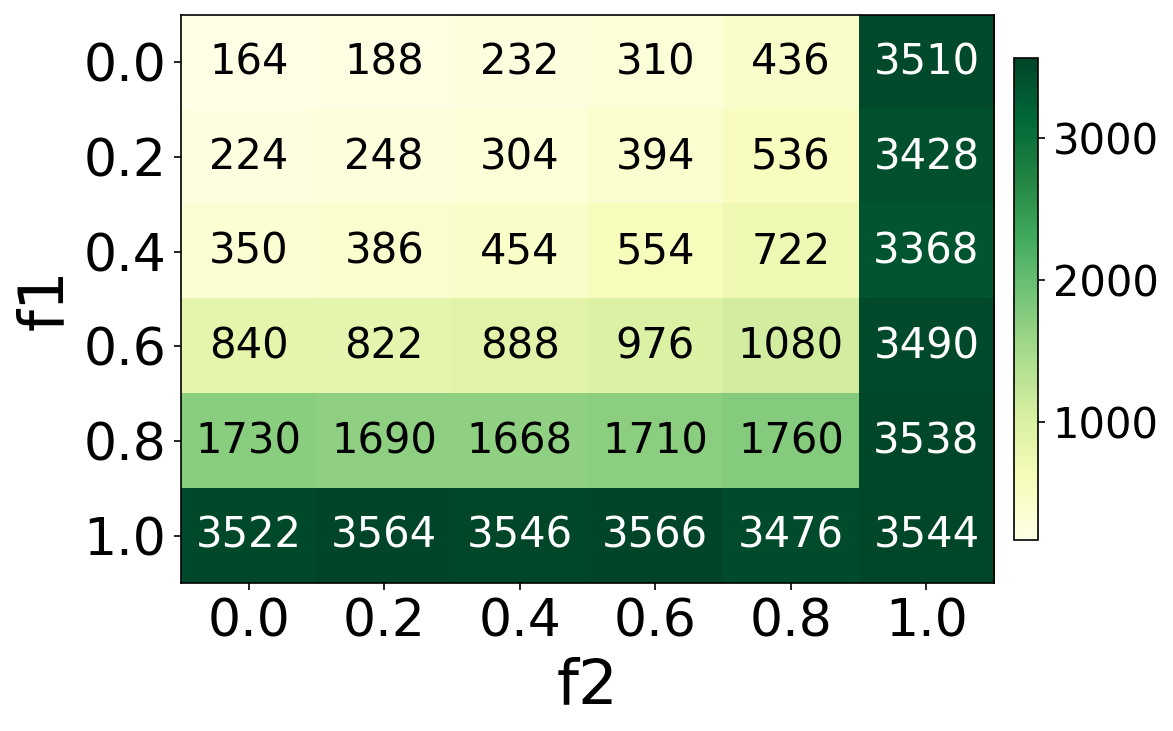
\includegraphics[width=\columnwidth]{results/tiered_prefix_sharing_plots/vllm_heatmap_throughput.png}
\caption{Throughput}
\label{fig:tp_tiered_prefix_sharing}
\end{subfigure}
\caption{Key Observations on Prefix Homogeneity}
\label{fig:tiered_prefix_sharing_fig}
\vspace{-15pt}
\end{figure}

\subsection{Key Observations on Prefix Homogeneity}
\label{subsec:tiered_prefix_sharing}
We consider an additional experiment where each request has a sequence length of $10K$ tokens. As illustrated in Figure~\ref{fig:vis_tiered_prefix_sharing}, a fraction $f_1 \in [0, 1]$ of this sequence is shared as a common prefix across all $500$ requests in the batch. The remaining $10K(1 - f_1)$ tokens constitute the suffix of each request. Within the batch, a fraction $f_2 \in [0, 1]$ of requests share an identical suffix, denoted as $A$. The remaining fraction $(1 - f_2)$ has suffixes drawn from one of $50$ distinct groups, $B_1, \dots, B_{50}$. Figure~\ref{fig:tp_tiered_prefix_sharing} presents the throughput as we vary $f_1$ and $f_2$. Consistent with the observations in \S\ref{subsec:significance_of_prefix_homogeneity}, increasing $f_1$ improves throughput due to enhanced temporal and spatial locality in KV cache accesses. Additionally, we observe a sharp increase in throughput when $f_2$ changes from $0.8$ to $1$. This occurs because at $f_2 = 1$, the entire batch becomes homogeneous, resulting in fully aligned KV cache traversal. Throughput is significantly lower at smaller values of $f_1$, primarily because limited GPU memory leads to frequent cache evictions. This is further supported by the increase in throughput with rising $f_2$ at low $f_1$, as more requests share the suffix $A$, reducing eviction frequency. However, once the working set fits within GPU memory (around $f_1 = 0.8$), throughput remains nearly constant for all $f_2 < 1$, indicating that residual heterogeneity has minimal impact. Overall, this experiment consolidates the key insights discussed in \S\ref{subsec:significance_of_prefix_homogeneity}.

\section{Operations of Chunked Hash Tree}
\label{sec:algorithms}
This section provides pseudo-codes and details of various algorithms used in the Chunked Hash Tree (\S\ref{subsec:chunked_hash_tree}).

\subsection{Variables and Notations}
Table~\ref{tab:cht_variables_and_notations} provides a list of all the variables and notations used in the following pseudo-codes.

\begin{table}[t]
\centering
\small
\resizebox{\columnwidth}{!}{\begin{tabular}{l p{0.8\columnwidth}}
\toprule
\textbf{Variable} & \textbf{Explanation} \\
\midrule
$T$      & Sequence length in tokens  \\
$C$      & Number of chunks in a sequence  \\
$K$      & Chunk size  \\
$H$      & Hash vector  \\
$r$      & Request  \\
$W$      & Number of waiting requests \\
$W_h$    & Average number of waiting requests sharing a hash \\
$(l^*, h^*)$ & Shared prefix tip \\
$h_l^r$ & Hash at level $l$ of request $r$ \\
$\texttt{working\_set}$ & Working set \\
$\texttt{waiting}$ & Reverse index from hashes to waiting requests \\
$\texttt{waiting\_heap}$ & Min-heap \\
$\texttt{request\_hashes}$ & Map from request to its hash vector \\
$\texttt{miss}$ & Map from request to its missing count \\
$\texttt{active}$ & Set of requests present in the current batch\\
$\texttt{waiting\_requests}$ & Set of waiting requests \\
$\texttt{ref}$ & Map from hash to number of active requests sharing it \\
\bottomrule
\end{tabular}}
\caption{Variables and Notations Used}
\label{tab:cht_variables_and_notations}
\vspace{-15pt}
\end{table}

\subsection{Prefix Hash Computation}
\label{subsec:chunked_hash_tree_prefix_representation}
The goal is to efficiently compute prefix-aligned hashes at fixed chunk boundaries. Algorithm~\ref{alg:compute_hashes} computes the hash vector for a token sequence using an incremental hashing scheme (Figure~\ref{fig:chunked_hash_tree_prefix_representation}). Instead of recomputing hashes for each prefix independently, the algorithm maintains a streaming hash state that is updated once per token. The algorithm processes each token exactly once and performs constant-time updates to the hash state. As a result, it runs in $\mathcal{O}(T)$ time and produces $C = \lceil T / K \rceil$ hash values, yielding $\mathcal{O}(C)$ output space. While Algorithm~\ref{alg:compute_hashes} processes tokens sequentially, the prefix-hash vector can equivalently be computed in parallel across chunks. The key property we want is that all requests sharing the first $c \cdot K$ tokens produce an identical $h_c$. This is achieved by partitioning the token sequence into chunks $S_c = (t_{(c-1)K+1}, \dots, t_{cK})$, hashing each chunk independently in parallel, and then chaining the results via $h_c = \textsc{Hash}(h_{c-1} \,\|\, \textsc{Hash}(S_c))$, with $h_0$ set to a fixed initialization constant (Algorithm~\ref{alg:compute_hashes_parallel}). With parallel workers, the dominant hashing phase runs in $\mathcal{O}(K)$ per worker rather than $\mathcal{O}(T)$ sequentially, reducing overall wall-clock time to $\mathcal{O}(K + C)$; the subsequent chaining pass costs only $\mathcal{O}(C)$ and is negligible in practice. This parallelization is most beneficial when $K$ is large, as each chunk contains more tokens and therefore represents a heavier independent unit of work, allowing parallel workers to amortize scheduling overhead across a larger payload and yielding greater absolute speedup over the sequential baseline. Both algorithms produce a hash vector satisfying the prefix-consistency property---all requests sharing the first $c \cdot K$ tokens yield the same $h_c$, yet the two vectors differ in their actual hash values, as Algorithm~\ref{alg:compute_hashes_parallel} is a distinct formulation rather than a parallelized execution of Algorithm~\ref{alg:compute_hashes}.

\begin{algorithm}[b]
\caption{\textsc{ComputeHashes}(S, K)}
\label{alg:compute_hashes}
\begin{algorithmic}[1]
\Require Token sequence $(t_1, \dots, t_T)$; chunk size $K$
\Ensure Cumulative prefix-hash vector $H = (h_1, \dots, h_C)$
\State $H \gets []$;\quad $C \gets \lceil T / K \rceil$
\State Initialise incremental \textsc{xxHash-64} state $s$
\For{$i \gets 1$ \textbf{to} $T$}
  \State Feed $t_i$ into $s$
  \If{$i \bmod K = 0$ \textbf{or} $i = T$}
    \State $H.\textsc{Append}(\textsc{Digest}(s))$
  \EndIf
\EndFor
\State \Return $H$
\end{algorithmic}
\end{algorithm}

\begin{algorithm}[t]
\caption{\textsc{ComputeHashesParallel}(S, K)}
\label{alg:compute_hashes_parallel}
\begin{algorithmic}[1]
\Require Token sequence $(t_1, \dots, t_T)$; chunk size $K$
\Ensure Cumulative prefix-hash vector $H = (h_1, \dots, h_C)$
\State $C \gets \lceil T / K \rceil$
\State $h_0 \gets \textsc{InitConst}$
\vspace{2pt}
\State \textbf{parallel for} $c \gets 1$ \textbf{to} $C$ \textbf{do} \Comment{Independent per-chunk hashes}
  \State \hspace{\algorithmicindent} $S_c \gets (t_{(c-1)K+1}, \dots, t_{\min(cK,\,T)})$
  \State \hspace{\algorithmicindent} $\ell_c \gets \textsc{Hash}(S_c)$ \Comment{Each chunk hashed independently}
\State \textbf{end parallel for}
\vspace{2pt}
\For{$c \gets 1$ \textbf{to} $C$} \Comment{Sequential prefix chaining}
  \State $h_c \gets \textsc{Hash}(h_{c-1} \,\|\, \ell_c)$
\EndFor
\State \Return $H = (h_1, \dots, h_C)$
\end{algorithmic}
\end{algorithm}

\begin{figure}[t]
\vspace{-10pt}
\centering
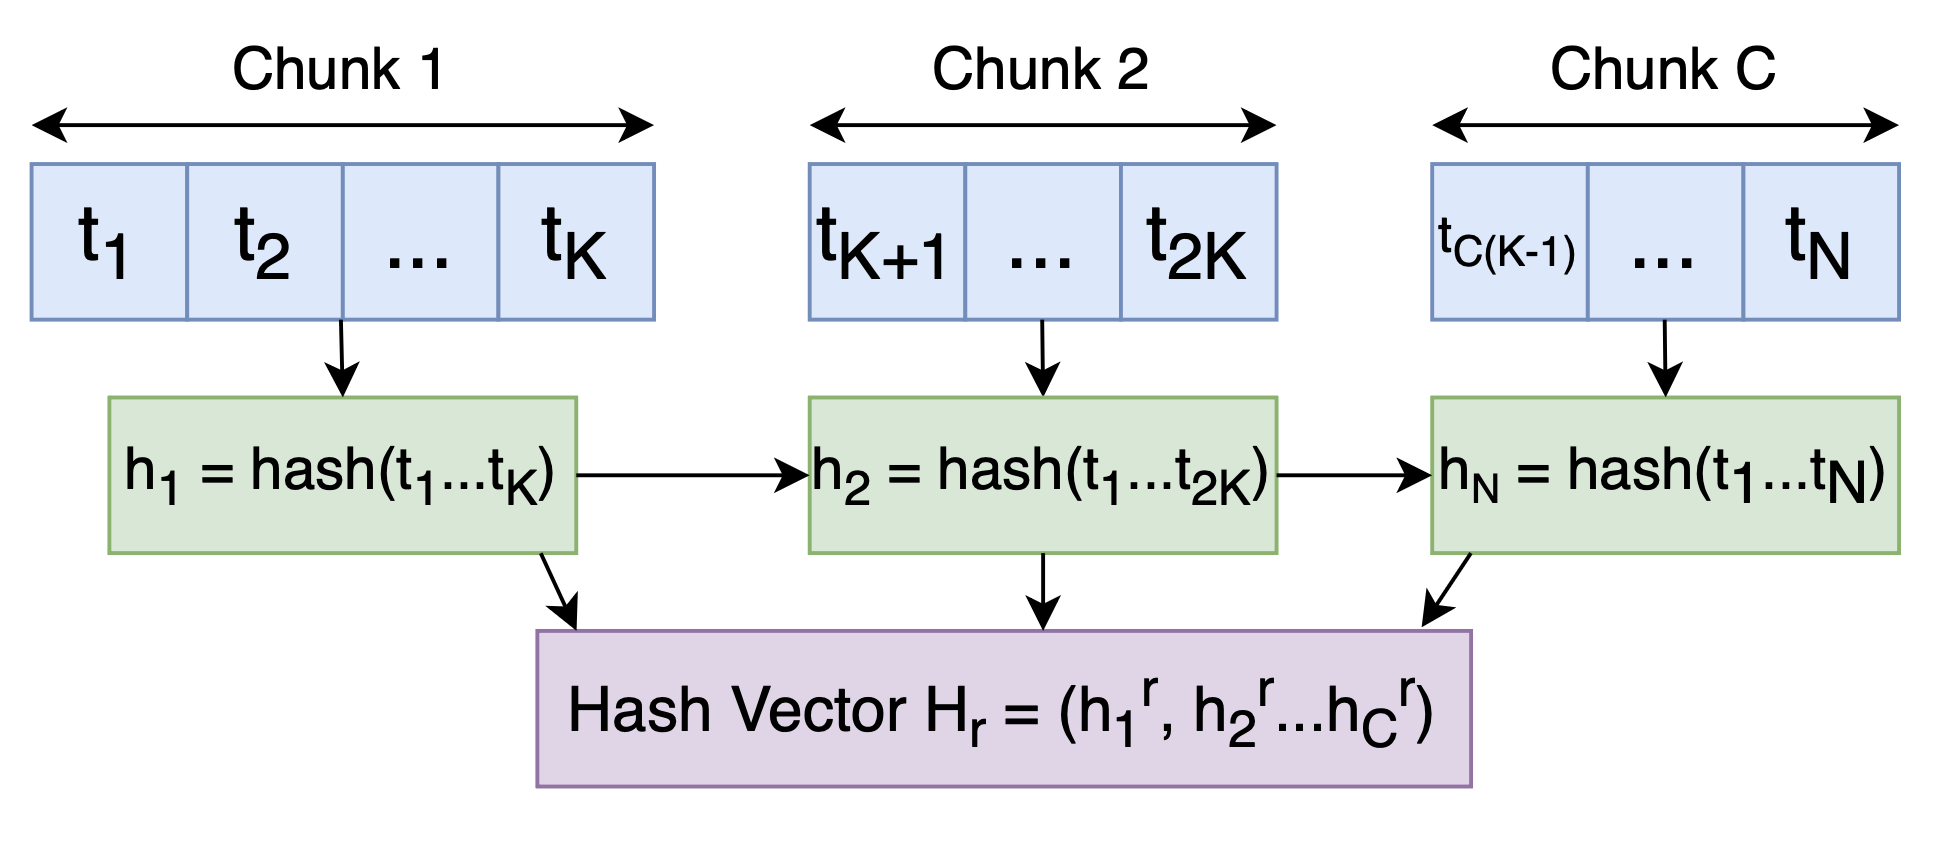
\includegraphics[width=0.7\columnwidth]{illustration_images/chunked_hash_tree_prefix_representation.png}
\caption{Hash Computation in Chunked Hash Tree}
\label{fig:chunked_hash_tree_prefix_representation}
\vspace{-10pt}
\end{figure}

\subsection{Insertion}
Algorithm~\ref{alg:insert} provides the pseudo-code for the \textsc{Insert} procedure. Given a request with a token sequence, we compute its cumulative prefix-hash vector using \textsc{ComputeHashes} and store it in a dictionary that maps each request to its hashes for easier reuse later (lines 1-2). For each level, we retrieve the corresponding hash and check whether the tuple is present in the working set; if not, the missing count is incremented (lines 6-7). Simultaneously, the request is inserted into the reverse index (line 9), which maps each hash to the set of waiting requests containing it and supports efficient lookup of prefix-sharing candidates. After processing all levels, we store the miss count in a map and insert the tuple of miss count and the request into the min-heap, which is keyed by missing count, enabling efficient retrieval of the most compatible request (lines 11-12). The design avoids any updates to the working set or reference counts during insertion, ensuring low overhead. 

\begin{algorithm}[t]
\caption{\textsc{Insert}(r, S)}
\label{alg:insert}
\begin{algorithmic}[1]
\Require $r$; token sequence $S$; $\mathit{working\_set}$; $\mathit{waiting}$; $\mathit{waiting\_heap}$
\Ensure $r$ registered and ready for scheduling
\State $H_r \gets \textsc{ComputeHashes}(S, K)$
\State $\mathit{request\_hashes}[r] \gets H_r$
\State $m_r \gets 0$
\For{$\ell \gets 1$ \textbf{to} $|H_r|$}
  \State $h \gets h_\ell^r$
  \If{$(\ell, h) \notin \mathit{working\_set}$}
    \State $m_r \gets m_r + 1$
  \EndIf
  \State $\mathit{waiting}[h] \gets \mathit{waiting}[h] \cup \{r\}$
\EndFor
\State $\mathit{miss}[r] \gets m_r$
\State $\mathit{waiting\_heap}.\textsc{Push}(m_r,\; r)$
\end{algorithmic}
\end{algorithm}

\subsection{Finding the Best Request}
The \textsc{FindBest} procedure selects the most compatible waiting request by querying the min-heap while skipping stale entries arising from lazy updates until a valid minimum is found (lines 6-8). Once a candidate is identified, it is reinserted into the heap for future activations in case the RL policy decides to add this request to the batch (line 9), and three quantities are computed without modifying the system state: the current tip depth, the prospective depth, and the number of peers sharing the resulting prefix. The prospective depth is obtained via a backward scan over the cumulative hash vector, selecting the deepest level such that the corresponding level-hash tuple exists in the working set, which corresponds to the least common ancestor with the active set under the current state. The peer count is computed by counting waiting requests whose hash at that level matches that of the candidate request. The result is cached and reused until either the working set or the waiting queue changes, avoiding redundant recomputation across repeated calls. If no valid request is found, the procedure returns $\bot$.

\begin{algorithm}[t] 
\caption{\textsc{FindBest}()} 
\label{alg:find_best} 
\begin{algorithmic}[1] 
\Require $\mathit{waiting\_heap}$; $\mathit{miss}$; $\mathit{active}$; tip $(\ell^*, h^*)$; $\mathit{working\_set}$; $\mathit{request\_hashes}$ 
\Ensure $(r^*,\; \ell^*_{\mathit{before}},\; \ell^*_{\mathit{after}},\; \mathit{peers})$ or $\bot$ 
\If{$\mathit{waiting\_requests} = \emptyset$}\ 
\Return $\bot$ 
\EndIf 
\If{$\mathit{cache\_valid}$}\ 
\Return $\mathit{cached\_result}$ 
\EndIf 
\While{$\mathit{waiting\_heap} \neq \emptyset$} 
\State $(m, r) \gets \mathit{waiting\_heap}.\textsc{Pop}()$ 
\If{$r \in \mathit{active}$ \textbf{or} $r \notin \mathit{miss}$ \textbf{or} $\mathit{miss}[r] \neq m$}\ 
\textbf{continue} 
\EndIf 
\State $r^* \gets r$;\quad $\mathit{waiting\_heap}.\textsc{Push}(m, r^*)$ \Comment{restore for future calls} 
\State $\ell^*_{\mathit{before}} \gets \ell^*$ 
\State $\ell^*_{\mathit{after}} \gets \ell$ where $\ell$ is the largest $\ell \leq \min(\ell^*, |H_{r^*}|)$ s.t. $(\ell, h_\ell^{r^*}) \in \mathit{working\_set}$ \State $\mathit{peers} \gets |\{w \in \mathit{waiting\_requests} : h_{\ell^*_{\mathit{after}}}^w = h_{\ell^*_{\mathit{after}}}^{r^*}\}|$ 
\State Cache and \Return $(r^*,\; \ell^*_{\mathit{before}},\; \ell^*_{\mathit{after}},\; \mathit{peers})$ 
\EndWhile 
\State \Return $\bot$ 
\end{algorithmic} 
\end{algorithm}

\subsection{Adding a Request to the Active Batch}
Given a request with its prefix-hash vector, the \textsc{AddToBatch} procedure promotes it to the active set (line 1) and updates the working set, reference counts, and other metadata in a single backward pass over the prefix-hash vector. For each level, if the reference count of the corresponding hash is zero (no other active request shares it), the level-hash tuple is inserted into the working set, and all corresponding waiting requests have their miss counts decremented and are reinserted into the waiting heap (lines 7-12). The reference counts are incremented at all levels (line 14). In parallel, the shared prefix tip is recomputed by tracking the deepest level at which the level-hash tuple remains in the working set; the first such match during the backward traversal determines the new tip (lines 15-17), while the loop continues to ensure that all state updates are applied. If this is the first active request, the tip is initialized directly to the end of its prefix-hash vector.

\begin{algorithm}[t]
\caption{\textsc{AddToBatch}(r)}
\label{alg:add_to_batch}
\begin{algorithmic}[1]
\Require $H_r$; $\mathrm{ref}$; $\mathit{working\_set}$; $\mathit{waiting}$; $\mathit{miss}$; $\mathit{waiting\_heap}$; tip $(\ell^*, h^*)$; $\mathit{active}$
\Ensure Updated $\mathrm{ref}$, $\mathit{working\_set}$, $\mathit{miss}$, $(\ell^*, h^*)$

\State $\mathit{active} \gets \mathit{active} \cup \{r\}$;\quad $\mathit{waiting\_requests} \gets \mathit{waiting\_requests} \setminus \{r\}$

\If{$|\mathit{active}| = 1$}
  \State $(\ell^*, h^*) \gets (|H_r|,\; h_{|H_r|}^r)$;\quad \Return
\EndIf

\State $\ell_{\mathrm{tip}} \gets \min(\ell^*,\; |H_r|)$;\quad $(\ell^*, h^*) \gets (0, \bot)$

\For{$\ell \gets |H_r|$ \textbf{downto} $1$}
  \If{$\mathrm{ref}[h_\ell^r] = 0$}
    \State $\mathit{working\_set} \gets \mathit{working\_set} \cup \{(\ell, h_\ell^r)\}$
    \For{$w \in \mathit{waiting}[h_\ell^r],\; w \notin \mathit{active}$}
      \State $\mathit{miss}[w] \mathrel{-}= 1$; 
      \State $\mathit{waiting\_heap}.\textsc{Push}(\mathit{miss}[w], w)$
    \EndFor
  \EndIf
  \State $\mathrm{ref}[h_\ell^r] \mathrel{+}= 1$
  \If{$\ell^* = 0$ \textbf{and} $\ell \leq \ell_{\mathrm{tip}}$ \textbf{and} $(\ell, h_\ell^r) \in \mathit{working\_set}$}
    \State $(\ell^*, h^*) \gets (\ell,\; h_\ell^r)$
    \Comment{Least common ancestor found; continue loop for remaining working set updates}
  \EndIf
\EndFor
\end{algorithmic}
\end{algorithm}

\subsection{Removing a Request from the Active Batch}
Given a completed request, the \textsc{Finish} procedure removes it from the active set (line 1) and updates the working set, reference counts, and other metadata. A forward pass over the prefix-hash vector decrements the reference count at each level (line 3); if it drops to zero, the level-hash tuple is removed from the working set, and all the corresponding waiting requests have their miss counts incremented and are reinserted into the min-heap (lines 4-10). After updating the working set, the shared prefix tip is recomputed by attempting to extend it forward: starting from the previous tip level, we check successive levels up to the minimum length among active requests and extend the tip whenever the reference count at that level equals the number of active requests, indicating agreement across all of them; the scan terminates at the first disagreement (lines 19-26). If the active set becomes empty, the tip is reset to $(0, \bot)$ (lines 12-14), and if only one request remains, the tip is set to its full length (lines 15-18). Finally, \textsc{Remove} is invoked to clean auxiliary structures such as the reverse index and the stored hash vector (line 27).

\begin{algorithm}[t]
\caption{\textsc{Finish}(r)}
\label{alg:finish}
\begin{algorithmic}[1]
\Require $H_r$; $\mathrm{ref}$; $\mathit{working\_set}$; $\mathit{waiting}$; $\mathit{miss}$; $\mathit{waiting\_heap}$; tip $(\ell^*, h^*)$; $\mathit{active}$
\Ensure Updated $\mathrm{ref}$, $\mathit{working\_set}$, $\mathit{miss}$, $(\ell^*, h^*)$

\State $\mathit{active} \gets \mathit{active} \setminus \{r\}$

\For{$\ell \gets 1$ \textbf{to} $|H_r|$}
  \State $\mathrm{ref}[h_\ell^r] \mathrel{-}= 1$
  \If{$\mathrm{ref}[h_\ell^r] = 0$}
    \State $\mathit{working\_set} \gets \mathit{working\_set} \setminus \{(\ell, h_\ell^r)\}$
    \For{$w \in \mathit{waiting}[h_\ell^r],\; w \notin \mathit{active}$}
      \State $\mathit{miss}[w] \mathrel{+}= 1$;
      \State $\mathit{waiting\_heap}.\textsc{Push}(\mathit{miss}[w], w)$
    \EndFor
  \EndIf
\EndFor

\If{$\mathit{active} = \emptyset$}
  \State $(\ell^*, h^*) \gets (0, \bot)$;\quad \Return
\EndIf
\If{$|\mathit{active}| = 1$}
  \State let $q$ be the sole element of $\mathit{active}$
  \State $(\ell^*, h^*) \gets (|H_q|,\; h_{|H_q|}^q)$;\quad \Return
\EndIf

\While{$\ell^* + 1 \leq \min_{q \in \mathit{active}} |H_q|$}
  \Comment{try to extend tip forward}
  \State $\ell \gets \ell^* + 1$
  \If{$\mathrm{ref}[h_\ell^{q_0}] = |\mathit{active}|$ for arbitrary $q_0 \in \mathit{active}$}
    \Comment{all active requests agree at level $\ell$}
    \State $(\ell^*, h^*) \gets (\ell,\; h_\ell^{q_0})$
  \Else
    \State \textbf{break}
  \EndIf
\EndWhile
\State \textsc{Remove}(r)
\Comment{cleans reverse index and request hashes}
\end{algorithmic}
\end{algorithm}

\subsection{Batch Formation}
\textsc{BuildBatch} describes the entire pipeline, where we incrementally construct a batch by repeatedly querying \textsc{FindBest} to obtain the most compatible candidate, along with summary statistics, which are combined with the current batch size to form the RL state (lines 3-6). A policy (heuristic, bandit, or Q-learning) maps this state to an action, either \textsc{Add} or \textsc{Stop} (line 7); if \textsc{Add} is selected, the request is activated via \textsc{AddToBatch} and appended to the batch; otherwise, the loop terminates (lines 8-10). The procedure continues until the waiting queue is exhausted or the policy decides to stop, after which the constructed batch is executed for one decode iteration to obtain the observed throughput (line 12). This throughput serves as the reward signal used to update the policy (line 13), with bandit methods updating their statistics and Q-learning applying a Bellman update with parameters $\alpha$ and $\gamma$, while heuristic policies incur no update.

\begin{algorithm}[t]
\caption{\textsc{BuildBatch}()}
\label{alg:rl_batch}
\begin{algorithmic}[1]
\Require Waiting queue $Q$; policy $\pi$ (heuristic, bandit, or Q-learning); discount $\gamma$; learning rate $\alpha$
\Ensure Batch $B$ ready for one decode iteration
\State $B \gets \emptyset$
\While{$Q \neq \emptyset$}
    \State $(r^*, c_{\mathrm{before}}, c_{\mathrm{after}}, w) \gets \textsc{FindBest}()$
    \If{$r^* = \bot$} \textbf{break} \EndIf
    \State $s \gets (|B|,\; \Delta = c_{\mathrm{before}} - c_{\mathrm{after}},\; w)$
    \State $a \gets \pi(s)$ \Comment{heuristic rule / UCB look-up / $\varepsilon$-greedy Q-table}
    \If{$a = \textsc{Stop}$} \textbf{break} \EndIf
    \State \textsc{AddToBatch}($r^*$); \quad $B \gets B \cup \{r^*\}$
\EndWhile
\State $\text{throughput}_{\mathrm{decode}} \gets \textsc{ExecuteBatch}(B)$
\State \textbf{Update} $\pi$ with observed reward $\text{throughput}_{\mathrm{decode}}$ \Comment{no-op for heuristic}
\State \Return $B$
\end{algorithmic}
\end{algorithm}

\subsection{Complexity Analysis}
Table~\ref{tab:complexity} summarizes the time complexity of each operation. Tip maintenance in \textsc{AddToBatch} and \textsc{Finish} is subsumed within their $\mathcal{O}(C \cdot W_h \cdot \log W)$ passes and adds no asymptotic cost. In practice, the dominant cost is miss-count propagation, which updates all affected waiting requests per working-set change. Result caching avoids redundant \textsc{FindBest} traversals between mutations, keeping scheduling overhead low. We present the time taken by individual functions for a particular experimental setup in \S\ref{subsec:time_taken_individual_functions_chunked_hash_tree}. 

\begin{table}[t]
\centering
\begin{tabular}{ll}
\hline
\textbf{Operation} & \textbf{Complexity} \\
\hline
\textsc{Insert}     & $\mathcal{O}(T + C \log W)$ \\
\textsc{AddToBatch}  & $\mathcal{O}(C \cdot W_h \cdot \log W)$ \\
\textsc{Finish}      & $\mathcal{O}(C \cdot W_h \cdot \log W)$ \\
\textsc{FindBest}    & $\mathcal{O}(\log W)$ amortized; $\mathcal{O}(1)$ cached \\
\textsc{Remove}      & $\mathcal{O}(C)$ \\
\hline
\end{tabular}
\caption{Time complexity of CHT scheduler operations}
\label{tab:complexity}
\vspace{-10pt}
\end{table}

\subsection{Find Best Request - Alternative Heuristic}
\label{subsec:find_best_reques_alternative_heuristic}
An intuitive alternative to using the missing count (which is based on the difference with the working set) is to select a waiting request that maximizes the depth of the current shared prefix tip. However, this approach has a subtle flaw: the tip is inherently bottlenecked by the most divergent active request, limiting future extension. Consider a scenario where Level 1 is shared by all requests, but Level 2 splits into three branches: one for $R_1$, one shared by $R_2$ and $R_3$, and one for $R_4$ (Figure~\ref{fig:find_best_request_different_approach_example}). If the active batch contains $R_1$ and $R_2$, the shared prefix tip is restricted to Level 1. Selecting based only on this tip makes $R_3$ and $R_4$ appear equally viable. If the scheduler admits $R_4$, the tip remains at Level 1; when $R_1$ finishes, the remaining requests ($R_2$ and $R_4$) lie on divergent branches, leaving the tip still stuck. Our Chunked Hash Tree avoids this by evaluating candidates against the full working set using the missing count $m_r$, rather than anchoring to the bottlenecked tip. The working set tracks all prefix chunks present in any active request. In the example, since $R_2$ is active, its Level 2 chunk is already in the working set. Thus, $R_3$ requires fewer missing chunks than $R_4$, i.e., $m_{R_3} < m_{R_4}$. Selecting $R_3$ preserves future overlap: although the immediate tip remains bottlenecked, once $R_1$ finishes and is removed via \textsc{Finish}, the remaining batch $\{R_2, R_3\}$ shares a deeper prefix, and the tip extends to Level 2. 

So, we have two ways to find the best waiting request to be added to the batch. One is based on the difference from the working set, and the other is based on the shared prefix tip. Next, we try to formalize the metrics on which both of these ways are based. Let $W$ be the hashes in the current working set, which can be defined as: $\cup_{r \in A}H^r$, where $A$ is the active set of requests and $H^r$ is the set of hashes for request $r$. CHT selects the request that has the minimum miss-count, which can be defined as $m_W(r) = |H^r \setminus W|$. The shared prefix tip is the deepest level shared by all the requests of the active batch, which can be defined as $\max\{\ell : \forall r \in A, (\ell, h_\ell^r) \in W\}$. The alternative heuristic selects the request that leads to the maximum depth of the shared prefix tip, which is equivalent to minimizing the number of hashes missing from the working set at or above the current tip for that request. Let $m_S(r) = |S \setminus H^r|$, where $S$ is the set of all hashes at or above the current tip level in the working set, i.e., $S = \{h : (\ell, h) \in W, \ell \leq \ell^*\}$, where $\ell^*$ is the current tip level. That is, $m_S(r)$ denotes the number of hash chunks present in $S$, but not present in the request $r$. Therefore, we explore the alternative heuristic that minimizes $m_S(r)$ instead of $m_W(r)$.

Let us assume that all the requests have a length of $C$ chunks, and the best requests emitted from the two metrics are $r_W$ and $r_S$, respectively. Let us also assume that the shared prefix tip is at level $\ell^*$. We aim to show that $m_S(r_W) = m_S(r_S)$, that is, the working set metric causes equal loss in the shared prefix tip, implying that $r_W$ does not lead to less depth in the shared prefix tip compared to $r_S$. Let us assume, to the contrary, that $m_S(r_S) < m_S(r_W)$. Now, we compare $m_W(r_W)$ and $m_W(r_S)$ and aim to show that $m_W(r_W) > m_W(r_S)$, which contradicts the fact that $r_w$ minimizes the metric $m_W$.

Since $S$ represents the shared prefix of all active requests up to depth $\ell^*$, the working set $W$ contains exactly one unique hash per level for all levels $\ell \leq \ell^*$, which constitutes the set $S$. This property dictates that if any request $x$ misses a hash in $S$ at some level $k < \ell^*$, its prefix diverges from the \textit{entire} active batch at level $k$. Consequently, due to the cumulative nature of the chunked hashes, $x$ cannot share any hashes with $W$ at any level $\geq k$. Specifically, if a request does not fully match the shared tip (i.e., $m_S(x) > 0$), it cannot overlap with any deeper divergent branches in $W$. For such a request, its overlap with the working set is exactly its overlap with the shared tip: $|H^x \cap W| = |H^x \cap S| = \ell^* - m_S(x)$. Using our contrary assumption $m_S(r_S) < m_S(r_W)$, we evaluate the cost of both requests under the working set metric, $m_W(x) = C - |H^x \cap W|$. We consider two cases for $r_S$: 

\noindent \textbf{Case 1:} $r_S$ fully matches the shared prefix tip ($m_S(r_S) = 0$). Since $r_S$ matches $S$ entirely, $|H^{r_S} \cap S| = \ell^*$. It may also overlap with deeper branches in $W$, meaning $|H^{r_S} \cap W| \geq \ell^*$. Therefore, its cost is $m_W(r_S) \leq C - \ell^*$. Because $m_S(r_W) > m_S(r_S) = 0$, $r_W$ diverges before the tip. As established, this means $|H^r_W \cap W| = \ell^* - m_S(r_W) < \ell^*$. Thus, $m_W(r_W) = C - |H^r_W \cap W| > C - \ell^*$. Combining these inequalities yields: $m_W(r_S) < m_W(r_W)$ (Figure~\ref{fig:alternative_heuristic_case1}).

\noindent \textbf{Case 2:} $r_S$ diverges before the shared prefix tip ($m_S(r_S) > 0$). Since $m_S(r_W) > m_S(r_S) > 0$, both requests diverge before $\ell^*$. Their overlap with the working set is strictly limited to their overlap with $S$. Thus, $|H^{r_S} \cap W| = \ell^* - m_S(r_S)$ and $|H^r_W \cap W| = \ell^* - m_S(r_W)$. Because $m_S(r_S) < m_S(r_W)$, it logically follows that $|H^{r_S} \cap W| > |H^r_W \cap W|$. Consequently: $m_W(r_S) < m_W(r_W)$ (Figure~\ref{fig:alternative_heuristic_case2}).

In both cases, assuming $m_S(r_S) < m_S(r_W)$ unavoidably leads to $m_W(r_S) < m_W(r_W)$. However, this directly contradicts our initial premise that $r_W$ is the optimal request chosen by the Chunked Hash Tree metric (which guaranties $m_W(r_W) \leq m_W(q)$ for all waiting requests $q$).  Therefore, our assumption must be false, proving that $m_S(r_W) \leq m_S(r_S)$. Because $r_S$ is defined as the absolute minimum for $m_S$, it must strictly hold that $m_S(r_W) = m_S(r_S)$. This completes the proof that optimizing for the working set metric is mathematically guaranteed to be at least as optimal as the shared prefix tip metric for preserving the immediate tip depth while simultaneously exposing deeper amortization opportunities in $W \setminus S$.

\begin{figure}[t]
\centering
    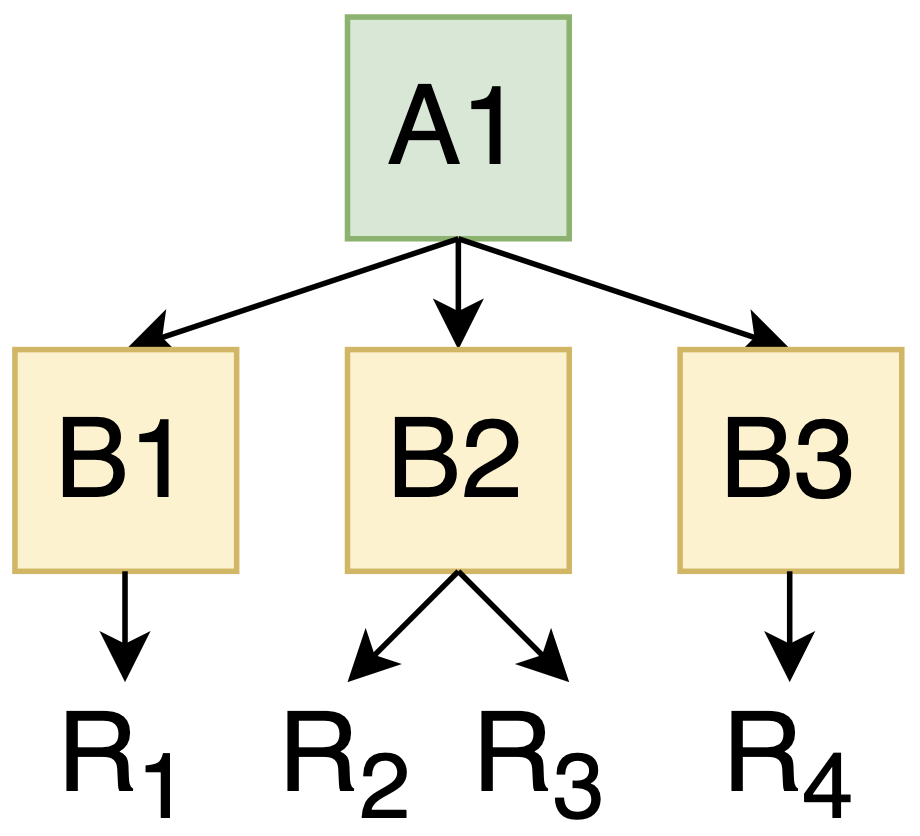
\includegraphics[width=0.25\linewidth]{illustration_images/find_best_request_different_approach_example.png}
    \caption{\textsc{FindBest} - Alternative Heuristic Example}
    \label{fig:find_best_request_different_approach_example}
    \vspace{-15pt}
\end{figure}

\begin{figure}[t]
\captionsetup[subfigure]{labelformat=simple}
    \renewcommand\thesubfigure{(\alph{subfigure})}
\centering
\begin{subfigure}{0.49\linewidth}
    \centering
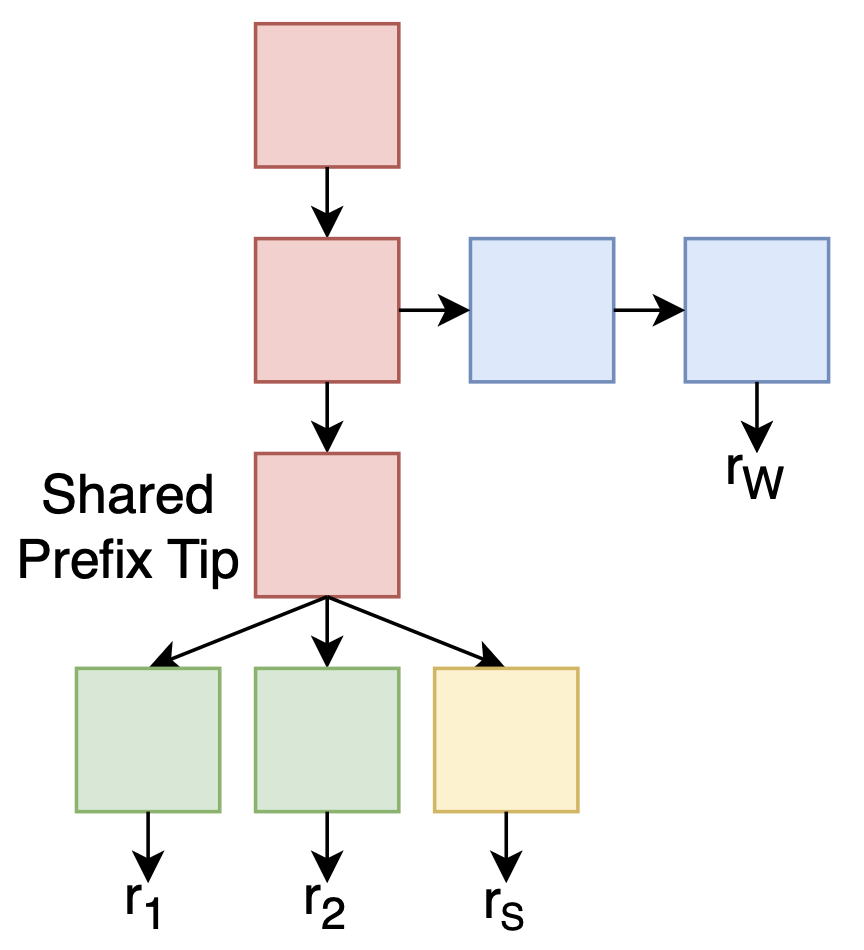
\includegraphics[width=\linewidth]{illustration_images/alternative_heuristic_case1.png}
\caption{Case 1}
\label{fig:alternative_heuristic_case1}
\end{subfigure}
\hfill
\begin{subfigure}{0.49\linewidth}
    \centering
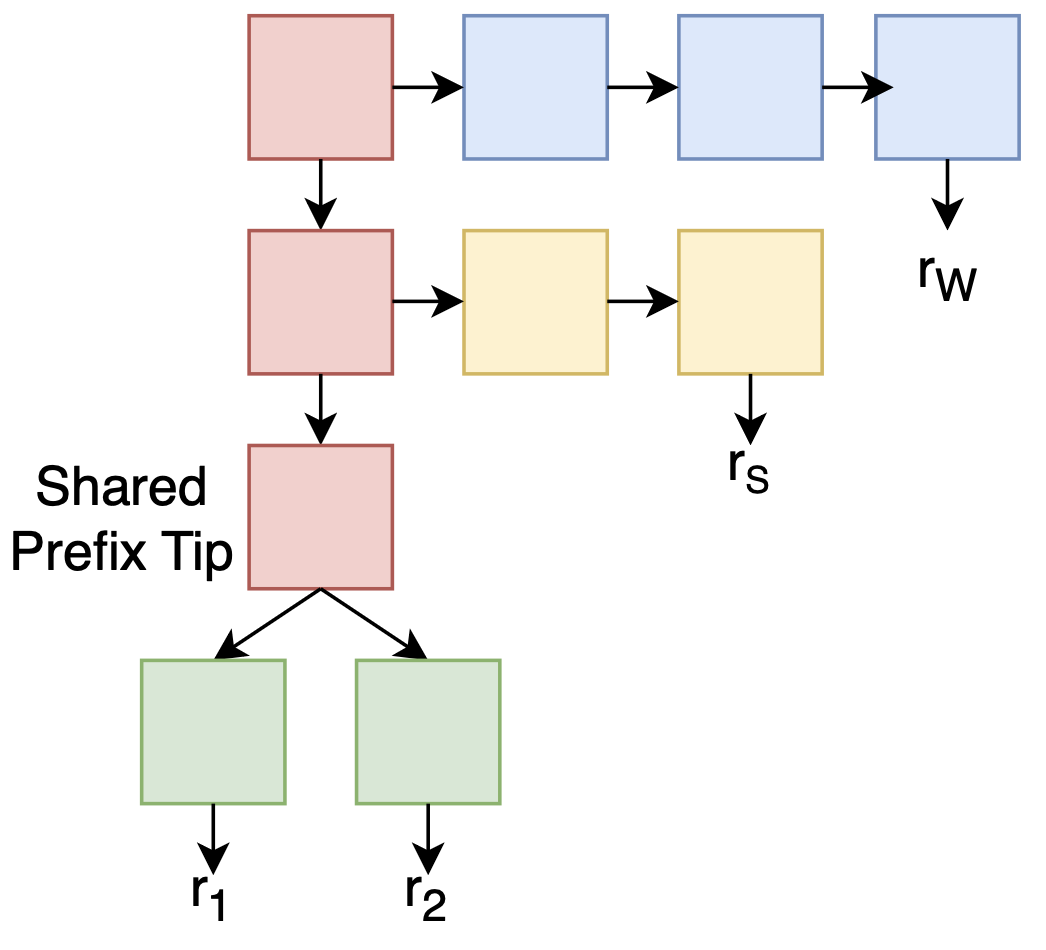
\includegraphics[width=\linewidth]{illustration_images/alternative_heuristic_case2.png}
\caption{Case 2}
\label{fig:alternative_heuristic_case2}
\end{subfigure}
\caption{\textsc{FindBest} cases: $r_1$ and $r_2$ are both present in the active batch, and hence the working set is the union of all of their chunks. The shared prefix tip is at the third level, and the set $S$ of all shared prefix chunks are marked in red. In the first case, $r_S$ fully matches the shared prefix tip, whereas $r_W$ hangs from the middle. For this case, $m_W(r_W) = 2, m_W(r_S) = 1, m_S(r_W) = 1, m_S(r_S) = 0$. In the second case, both the requests $r_S$ and $r_W$ do not fully match the shared prefix tip, however $r_W$ hangs off from an earlier chunk. For this case, $m_W(r_W) = 3, m_W(r_S) = 2, m_S(r_W) = 2, m_S(r_S) = 1$. Therefore, for both the cases, $m_W$ and $m_S$ exhibit similar behaviour.}
\label{fig:alternative_heuristic_cases}
\vspace{-10pt}
\end{figure}


\begin{figure*}[t]
\captionsetup[subfigure]{labelformat=simple}
    \renewcommand\thesubfigure{(\alph{subfigure})}
\centering
\begin{subfigure}{0.32\textwidth}
    \centering
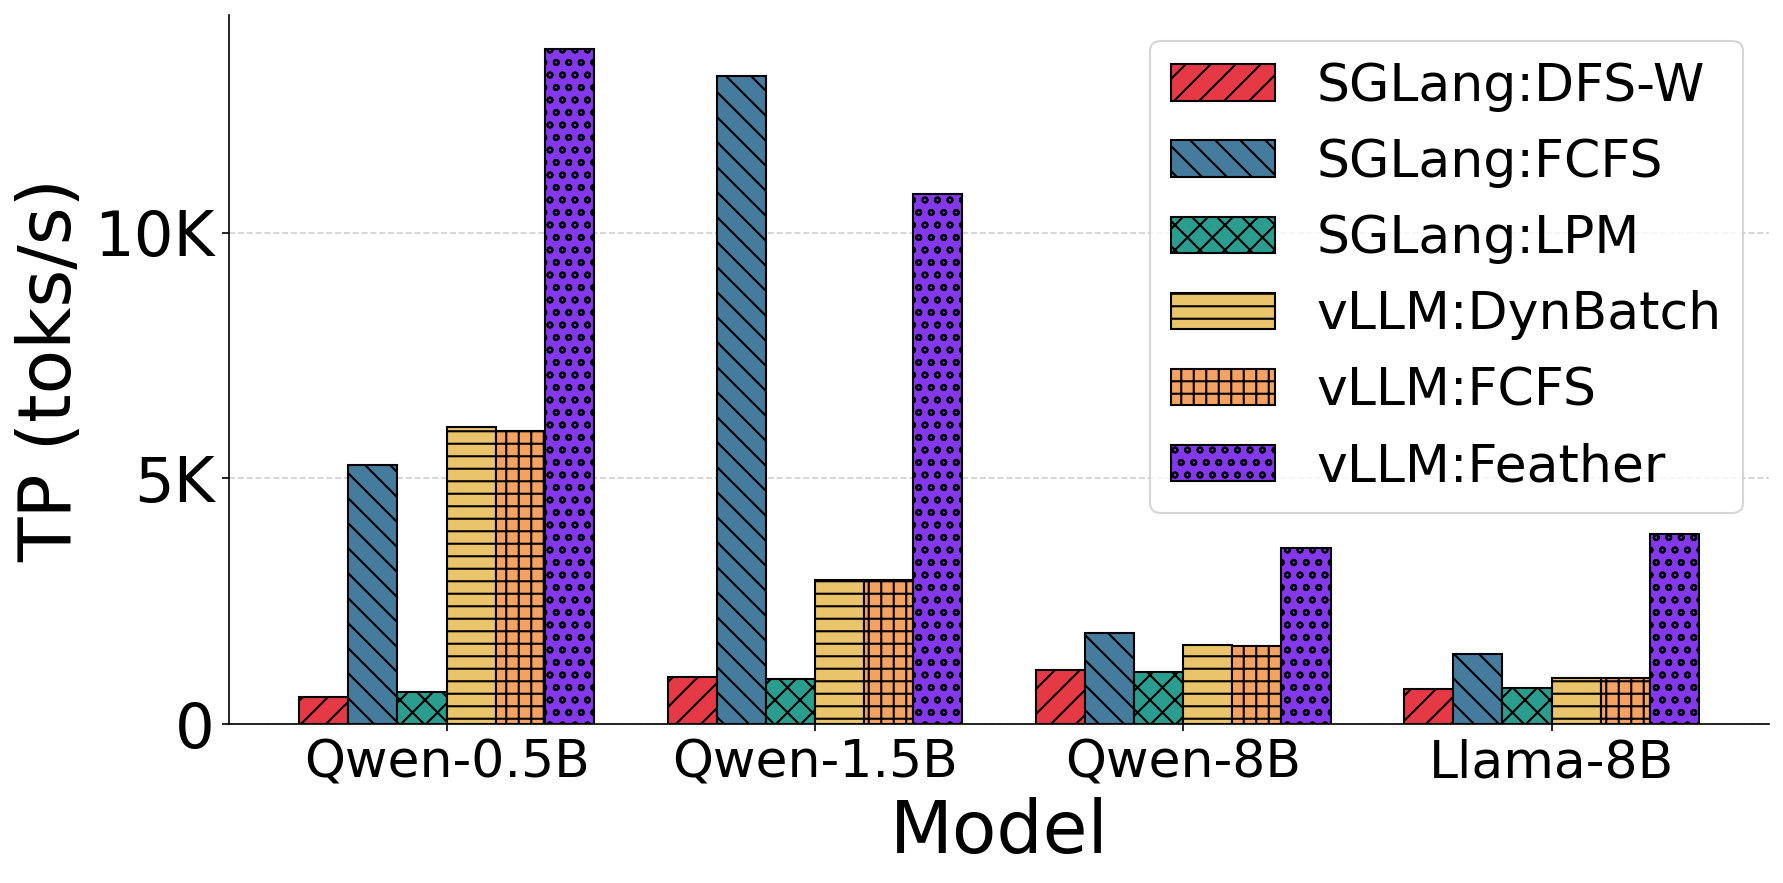
\includegraphics[width=\linewidth]{results/model_bar_plots/throughput_model_bar.png}
\caption{Throughput}
\label{fig:tp_vs_mod}
\end{subfigure}
\hfill
\begin{subfigure}{0.32\textwidth}
    \centering
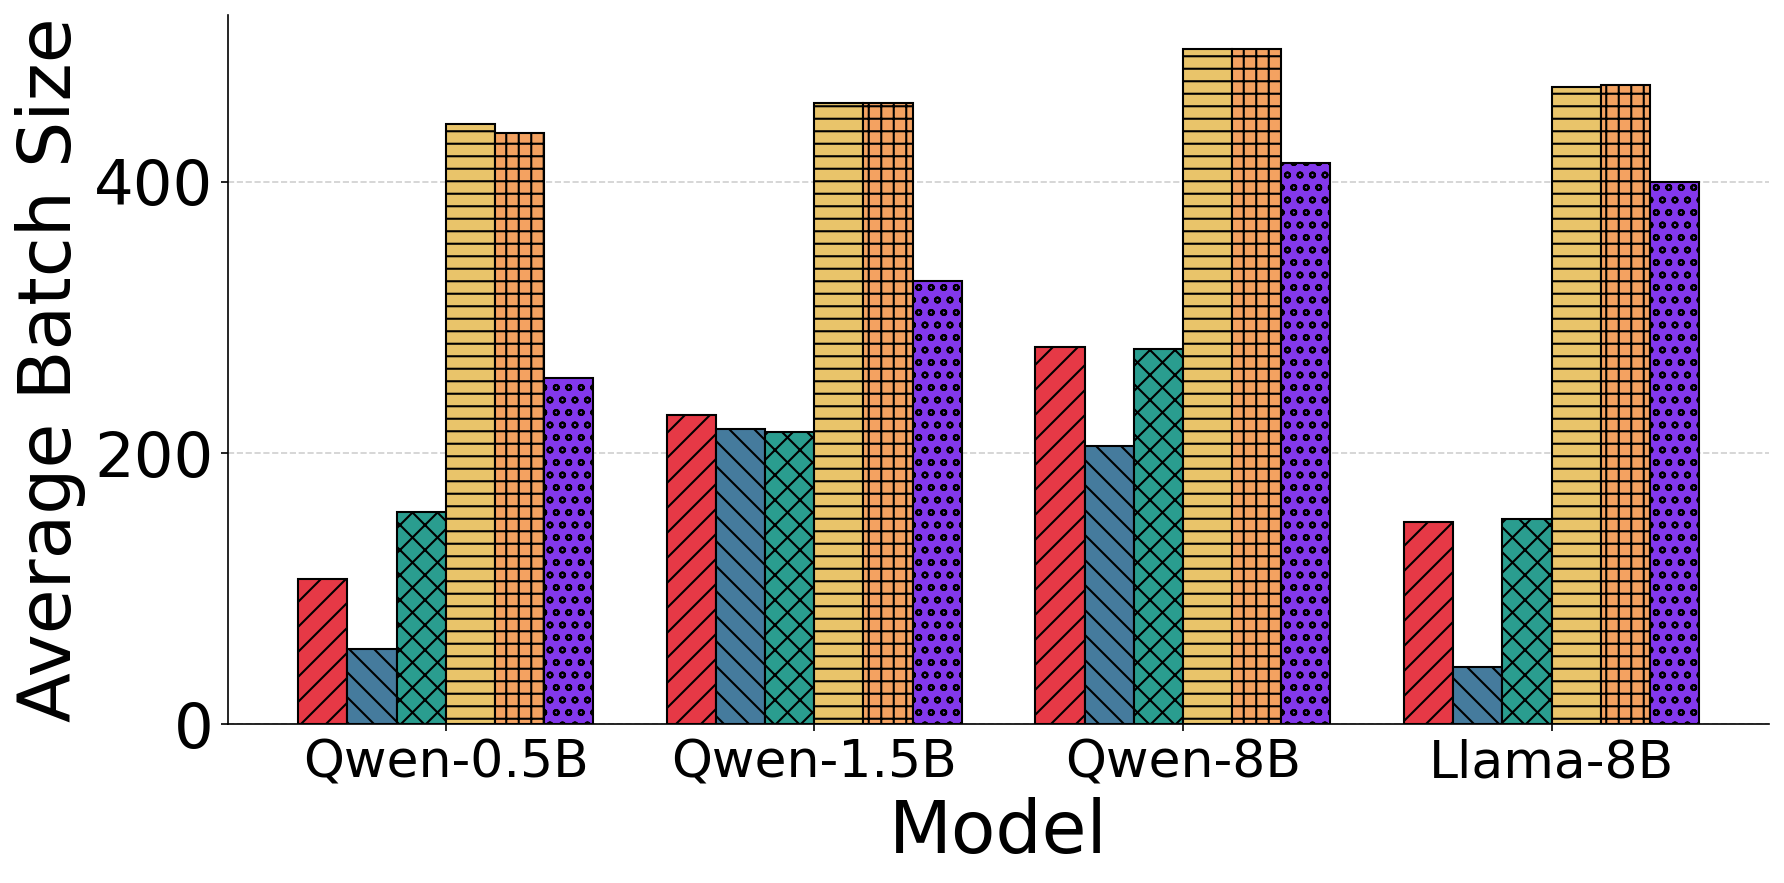
\includegraphics[width=\linewidth]{results/model_bar_plots/avg_batch_model_bar.png}
\caption{Average running batch size}
\label{fig:abs_vs_mod}
\end{subfigure}
\hfill
\begin{subfigure}{0.32\textwidth}
    \centering
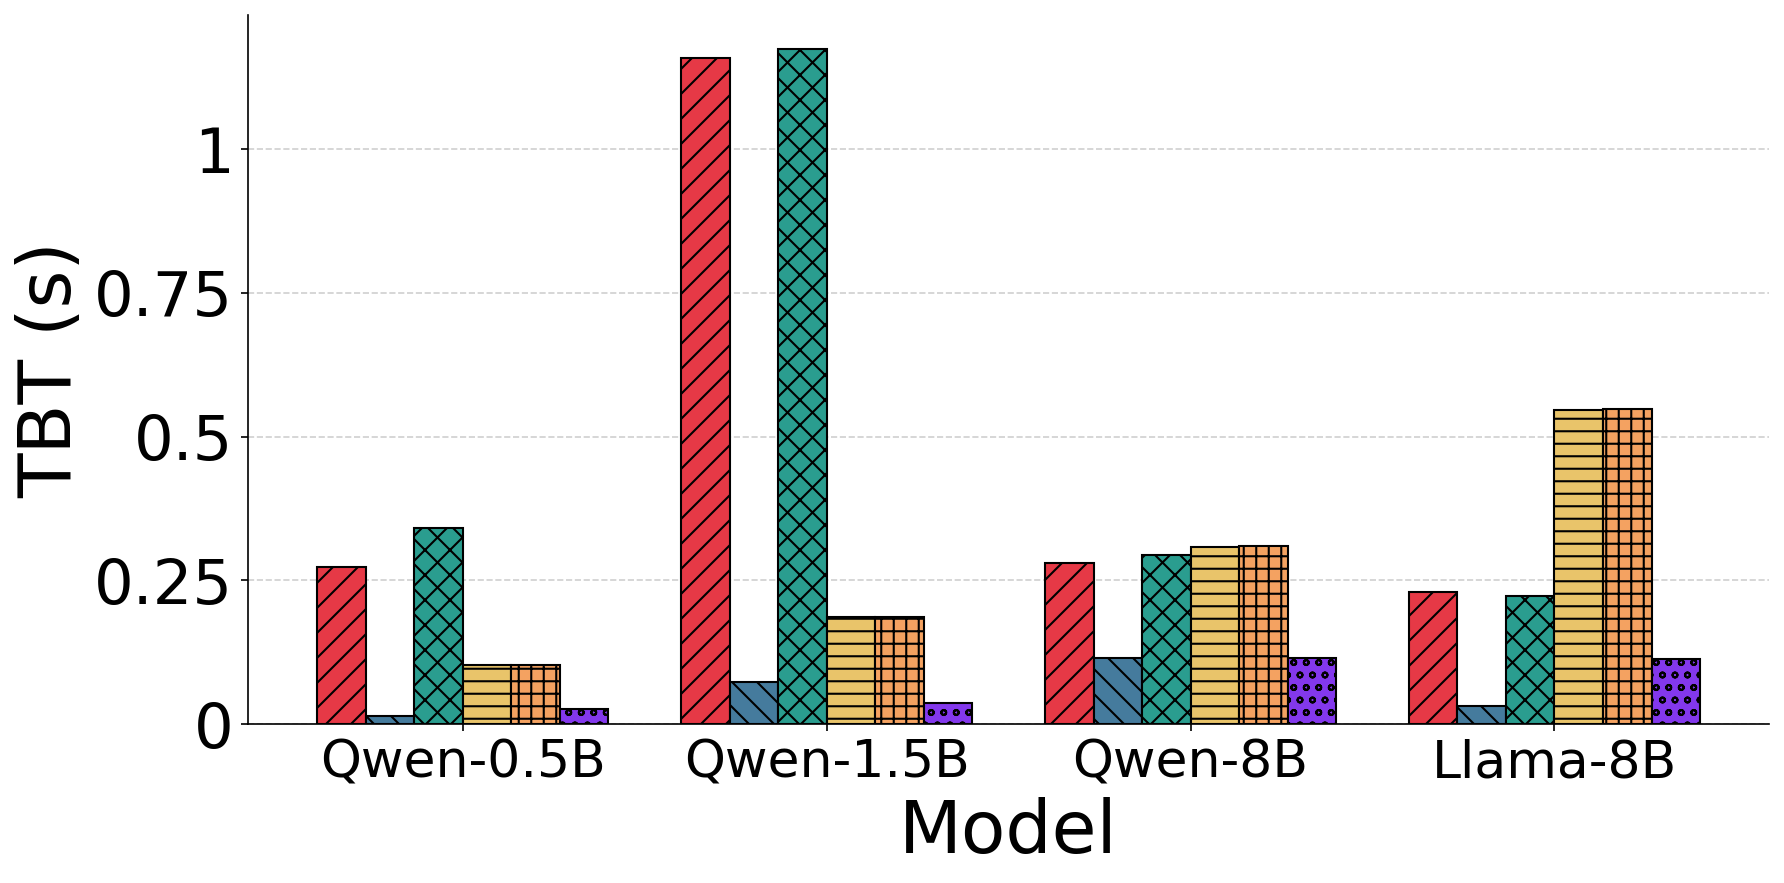
\includegraphics[width=\linewidth]{results/model_bar_plots/avg_timediff_model_bar.png}
\caption{Time between tokens (TBT)}
\label{fig:tbt_vs_mod}
\end{subfigure}
\caption{Different Models}
\label{fig:models}
\vspace{-10pt}
\end{figure*}

\begin{figure*}[t]
\captionsetup[subfigure]{labelformat=simple}
    \renewcommand\thesubfigure{(\alph{subfigure})}
\centering
\begin{subfigure}{0.30\linewidth}
    \centering
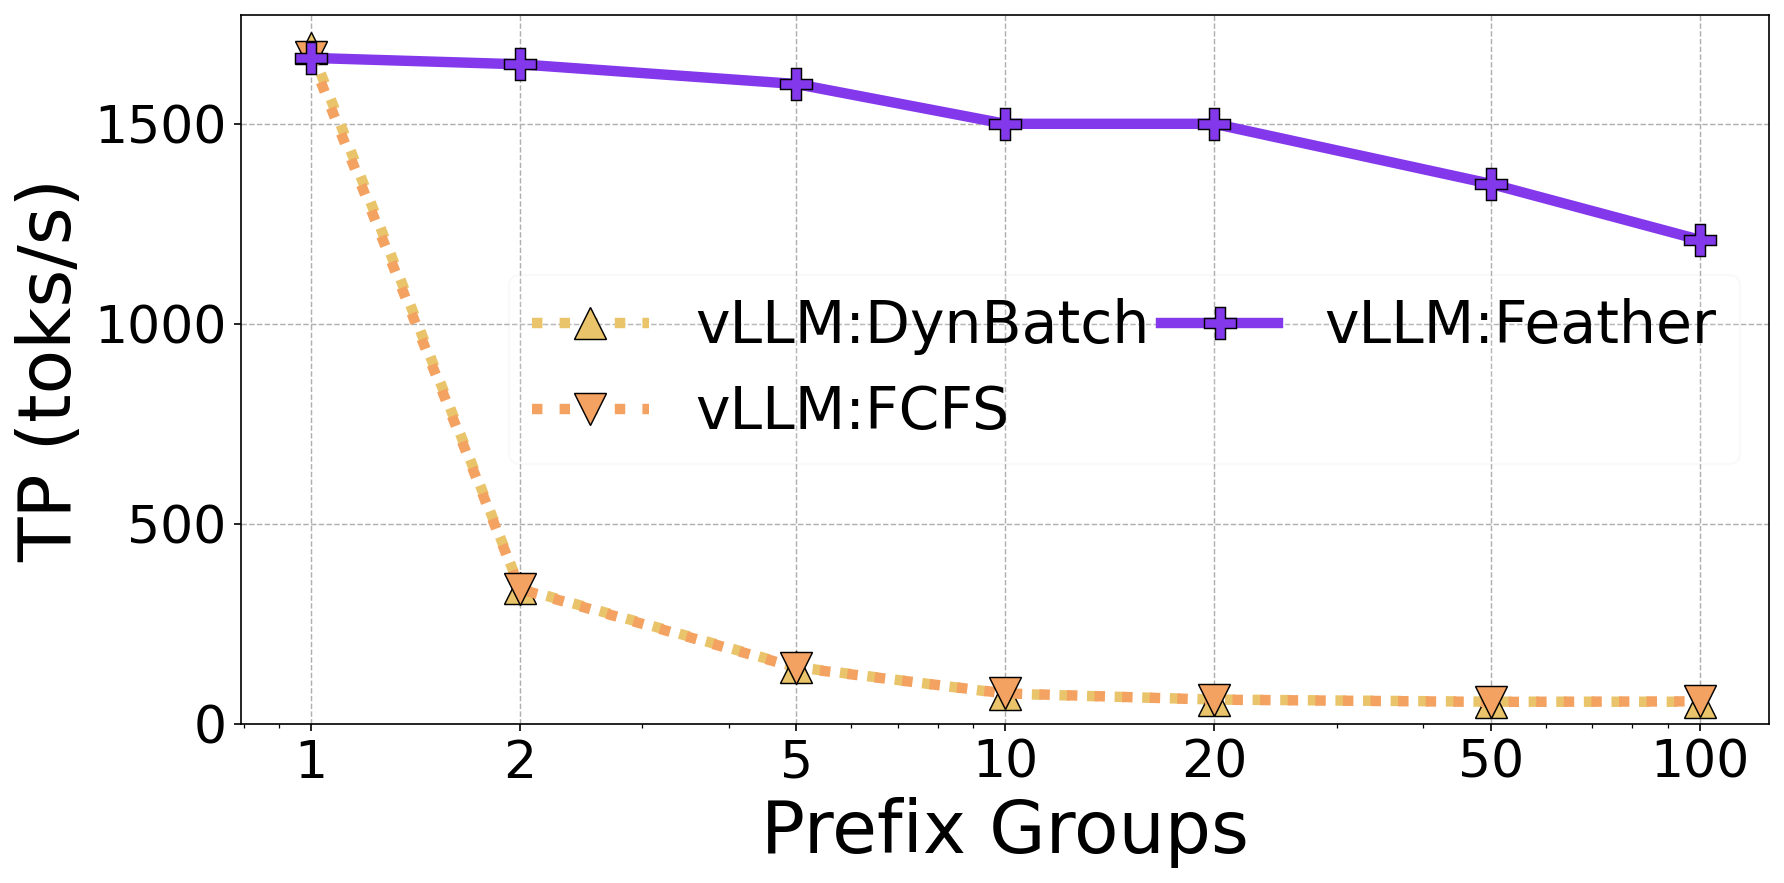
\includegraphics[width=\linewidth]{results/longchat_families_plots/throughput_vs_fam.png}
\caption{Throughput}
\label{fig:tp_vs_pref_long}
\end{subfigure}
\hfill
\begin{subfigure}{0.30\linewidth}
    \centering
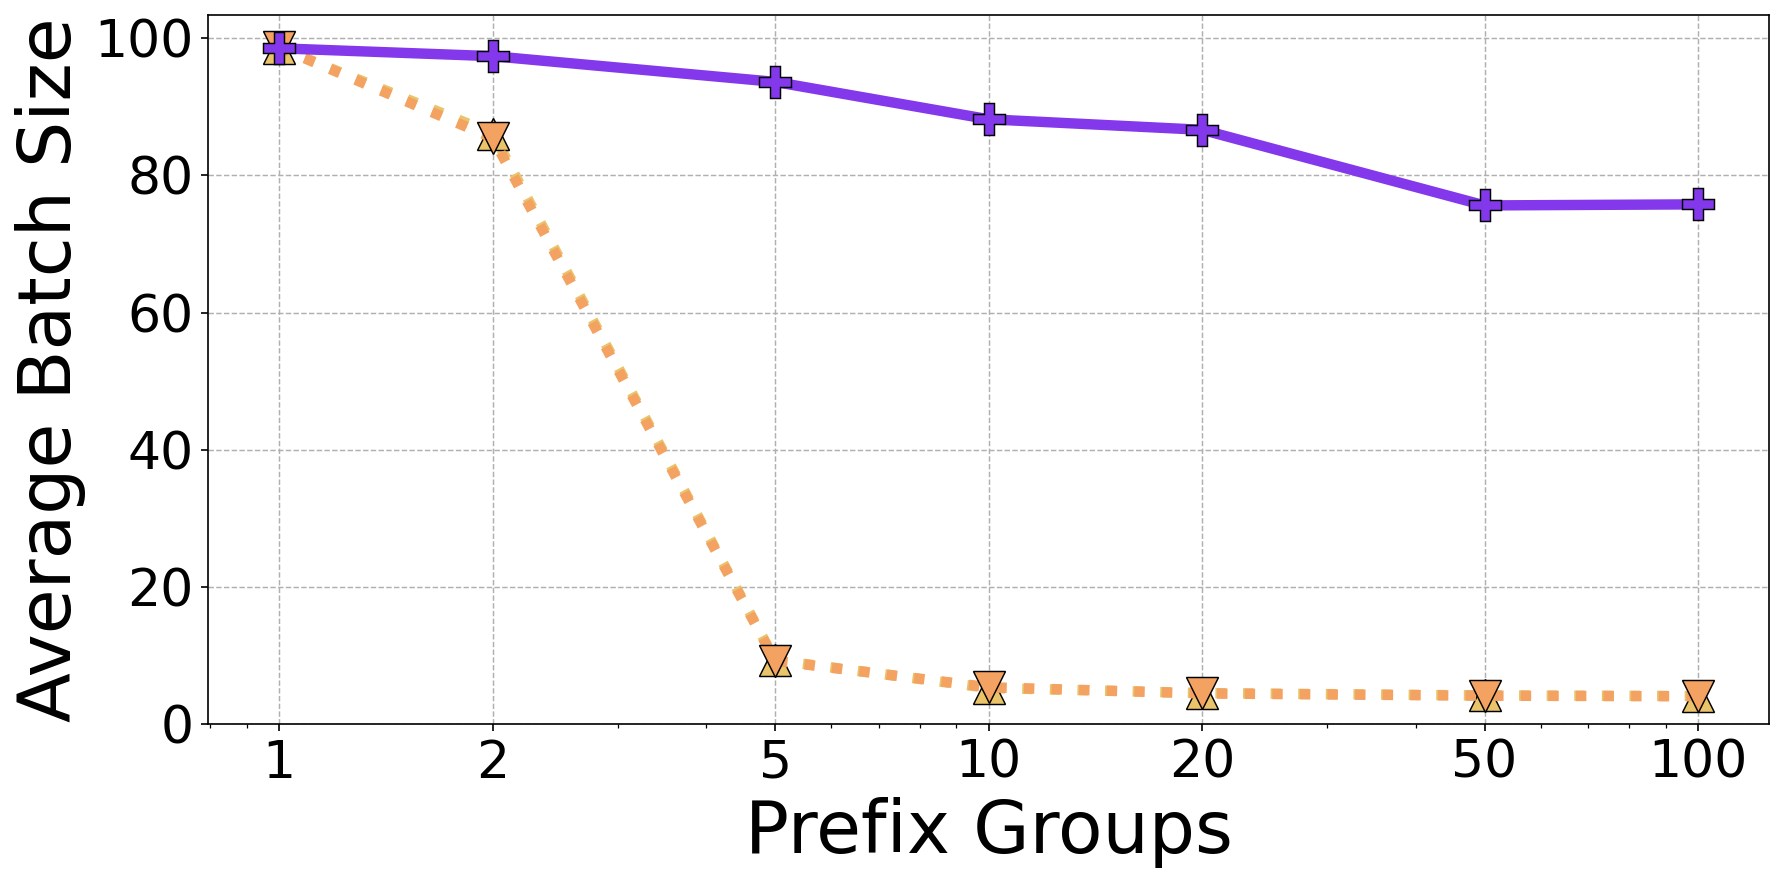
\includegraphics[width=\linewidth]{results/longchat_families_plots/avg_batch_vs_fam.png}
\caption{Average Batch Size}
\label{fig:abs_vs_pref_long}
\end{subfigure}
\hfill
\begin{subfigure}{0.30\linewidth}
    \centering
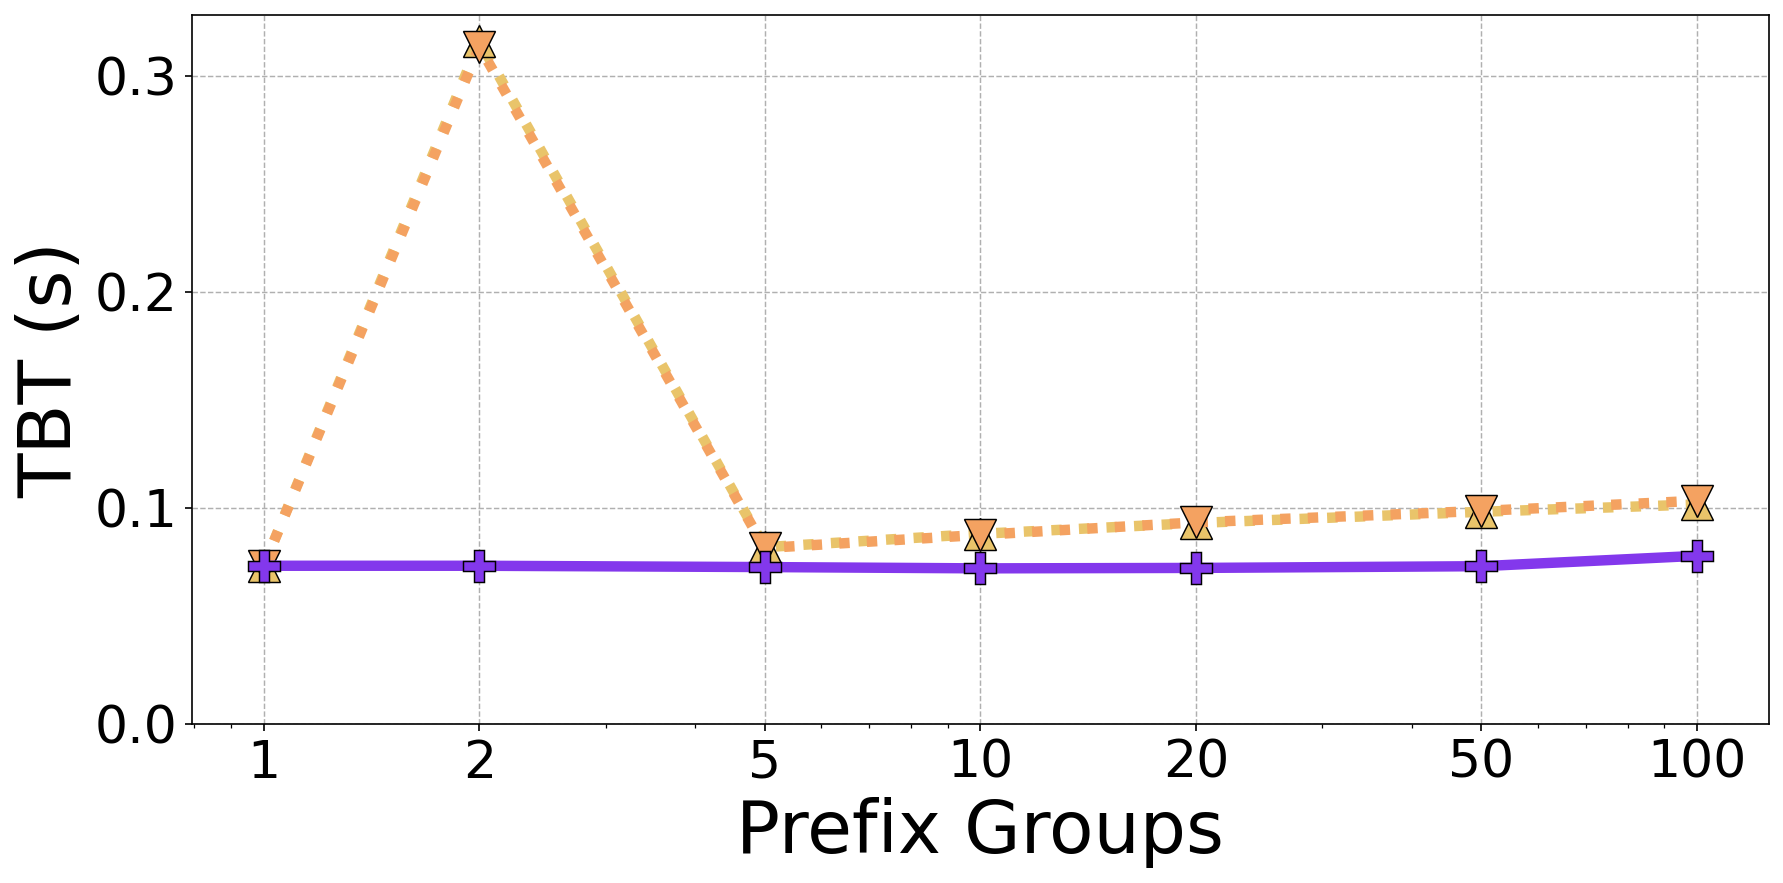
\includegraphics[width=\linewidth]{results/longchat_families_plots/avg_timediff_vs_fam.png}
\caption{Time between tokens (TBT)}
\label{fig:tbt_vs_pref_long}
\end{subfigure}
\caption{Varying number of prefix groups for LongChat 13B}
\label{fig:longhcat_results}
\vspace{-10pt}
\end{figure*}

\section{Additional Results of \Feather}
\label{sec:additional_results_of_feather}
Below, we present additional evaluation results of \Feather\ that could not be included in the main body due to space constraints.

\subsection{Time Taken by Individual Functions of CHT}
\label{subsec:time_taken_individual_functions_chunked_hash_tree}
Table~\ref{tab:chunked_hash_tree_individual_functions} profiles CHT operations over an inference workload of $5K$ requests, each $5K$ tokens long. \textsc{Insert}, \textsc{AddToBatch}, and \textsc{Finish} are each invoked $5K$ times, once per request. \textsc{FindBest}, however, is called $26{,}405$ times because it is queried repeatedly during batch construction. The RL policy may reject candidates and trigger fresh lookups, and the scheduler may inspect the queue multiple times before committing to a \textsc{Stop}. \textsc{Insert} dominates total time because hash computation scans every token once, making it proportional to prompt length. \textsc{Finish} is more expensive than \textsc{AddToBatch}, despite their symmetric roles. This gap arises from \textsc{Finish}'s additional forward tip-extension scan. After updating the working set, it traverses forward, level by level, to check if the shared prefix can be extended. In contrast, \textsc{AddToBatch} performs an early-terminating backward LCA scan, avoiding this overhead. \textsc{FindBest} is the cheapest per-call operation due to result caching and lazy heap traversal.

\begin{table}[t]
\centering
\small
\resizebox{\columnwidth}{!}{\begin{tabular}{lccc}
\toprule
\textbf{Function} & \textbf{Number of Calls} & \textbf{Average Time (ns)} & \textbf{Total Time (ns)} \\
\midrule
\textsc{Insert}      & 5,000  & 153,714 & 768,570,573 \\
\textsc{AddToBatch}  & 5,000  &  11,143 &  55,715,469 \\
\textsc{Finish}      & 5,000  &  38,952 & 194,760,111 \\
\textsc{FindBest}    & 26,405 &   6,641 & 175,372,986 \\
\bottomrule
\end{tabular}}
\caption{Time taken by individual functions of CHT}
\label{tab:chunked_hash_tree_individual_functions}
\vspace{-20pt}
\end{table}


\subsection{Performance of \Feather across Models}
\label{subsec:across_models}
Figures~\ref{fig:tp_vs_mod}, \ref{fig:abs_vs_mod}, \ref{fig:tbt_vs_mod} present throughput, average running batch size, and time between tokens (TBT) across models of varying sizes. The overall trend is consistent with expectations: smaller models achieve higher throughput owing to lower per-token compute costs. \Feather outperforms all baselines across all models. The sole exception is Qwen-1.5B, where SGLang FCFS achieves marginally higher throughput; however, \Feather compensates on the latency axis, exhibiting substantially lower TBT for the same model. A key structural observation is that \Feather's relative throughput advantage over the baselines grows with model size. As model size increases, a larger fraction of the total execution time is spent on attention computation, which amplifies the benefits of temporal and spatial KV-cache locality that \Feather exploits. This effect is visible in Figure~\ref{fig:tp_vs_mod}: the gap between \Feather and the next-best baseline widens from Qwen-0.5B to the 8B-scale models. The performance of SGLang's LPM and DFS-W schedulers degrades noticeably for smaller models. Both policies rely on CPU-side tree traversal, whose overhead scales with sequence length rather than model size; as the model shrinks, GPU execution time decreases while scheduler overhead remains roughly constant, causing the CPU to become an increasing bottleneck. \Feather avoids this through its Chunked Hash Tree, which reduces per-step scheduler complexity and keeps CPU overhead negligible relative to GPU execution time across all model scales. Finally, Figure \ref{fig:tbt_vs_mod} highlights that vLLM's FCFS and DB baselines incur substantially higher TBT at larger model sizes, whereas Feather keeps TBT low and stable. 

\subsection{Results across LongChat Model}
\label{subsec:results_across_longchat_model}
Figure~\ref{fig:longhcat_results} presents throughput, average batch size, and time between tokens (TBT) as the number of prefix groups varies for the LongChat 13B model. Overall, vLLM's FCFS and Dynamic Batching behave similarly across most configurations. For FCFS, there is a sharp drop in throughput when moving from 1 to 2 prefix groups, accompanied by an increase in TBT. This is largely due to the loss of locality benefits. The further decline from 2 to 5 prefix groups is driven by KV cache evictions, which is also reflected in the steep reduction in average batch size. Beyond this point, TBT stabilizes at a lower value, primarily because the batches have become much smaller. In contrast, \Feather maintains stable and consistent throughput across all settings. At 100 prefix groups, it achieves up to 22$\times$ higher throughput than FCFS. By forming prefix-homogeneous batches, \Feather not only improves scheduling efficiency but also significantly reduces KV cache evictions through more effective immediate cache reuse.

\begin{figure*}[t]
\captionsetup[subfigure]{labelformat=simple}
    \renewcommand\thesubfigure{(\alph{subfigure})}
\centering
\begin{subfigure}{0.30\linewidth}
    \centering
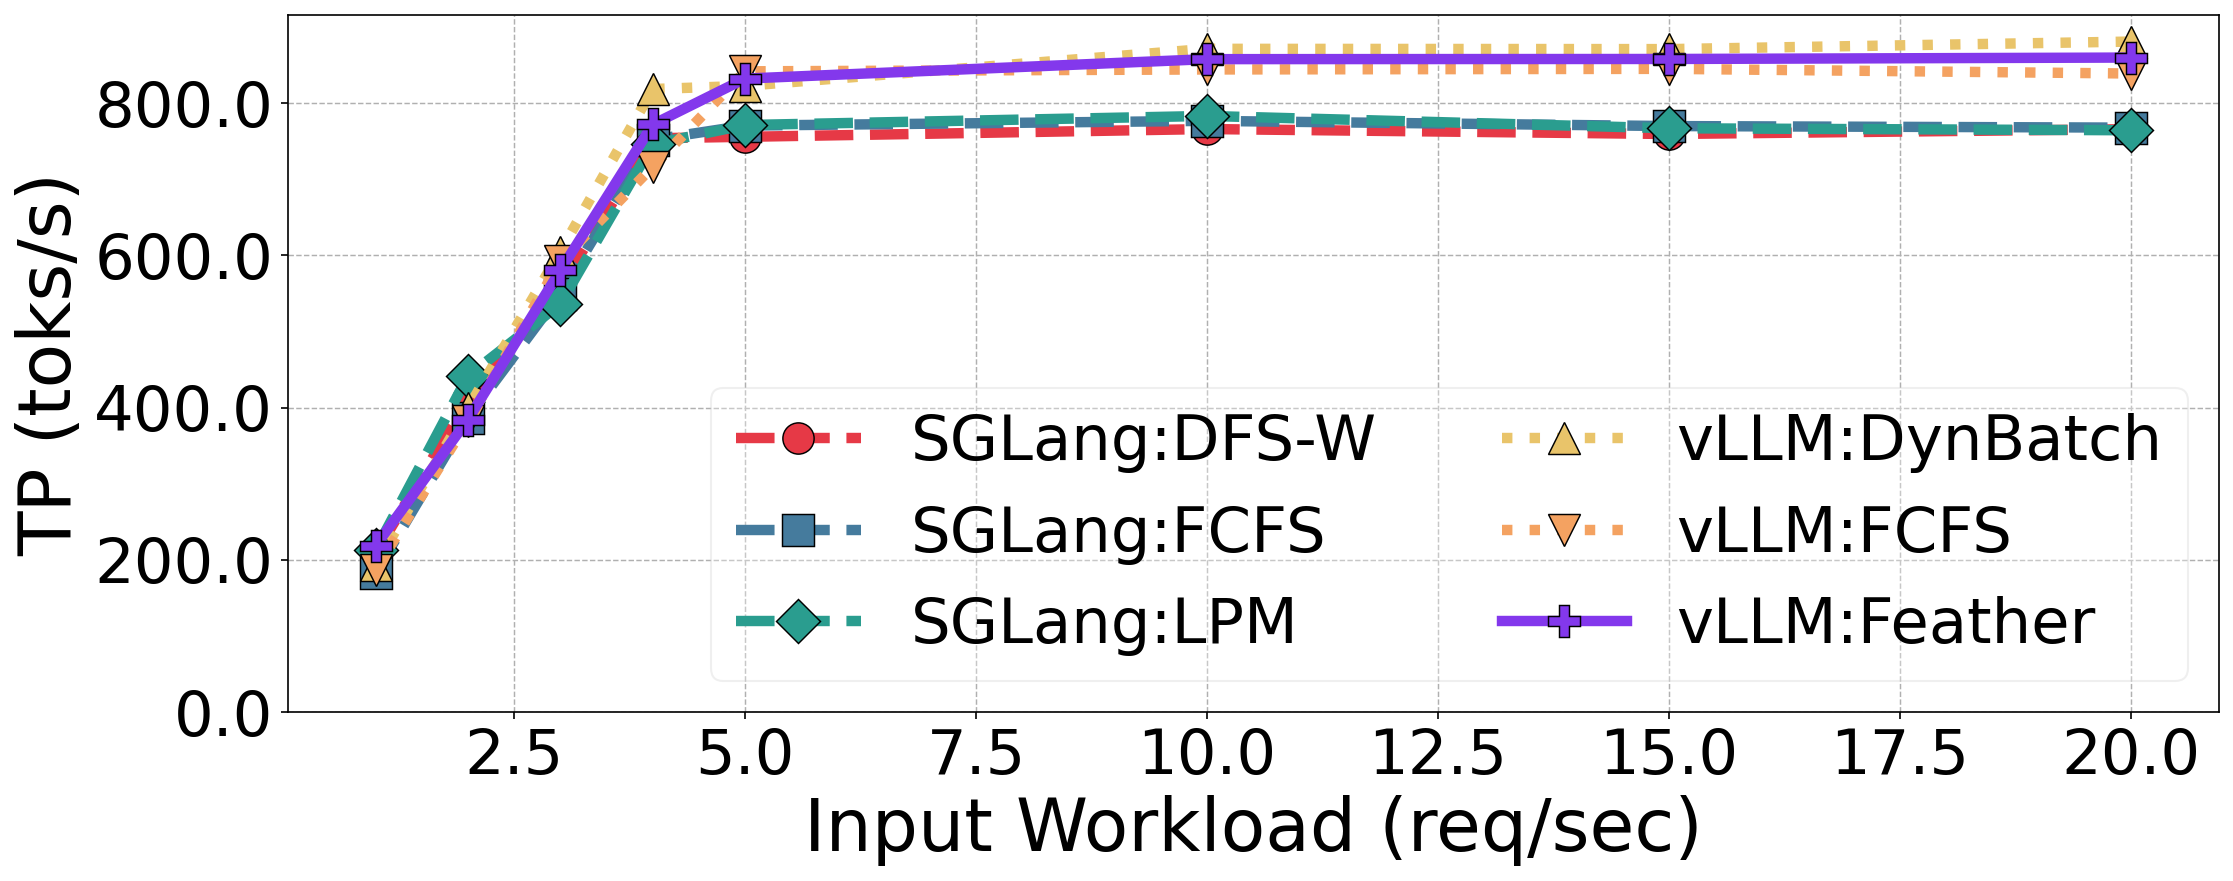
\includegraphics[width=\linewidth]{results/no_pref_sharing_plots/throughput_vs_rps.png}
\caption{Throughput}
\label{fig:tp_no_pref}
\end{subfigure}
\hfill
\begin{subfigure}{0.30\linewidth}
    \centering
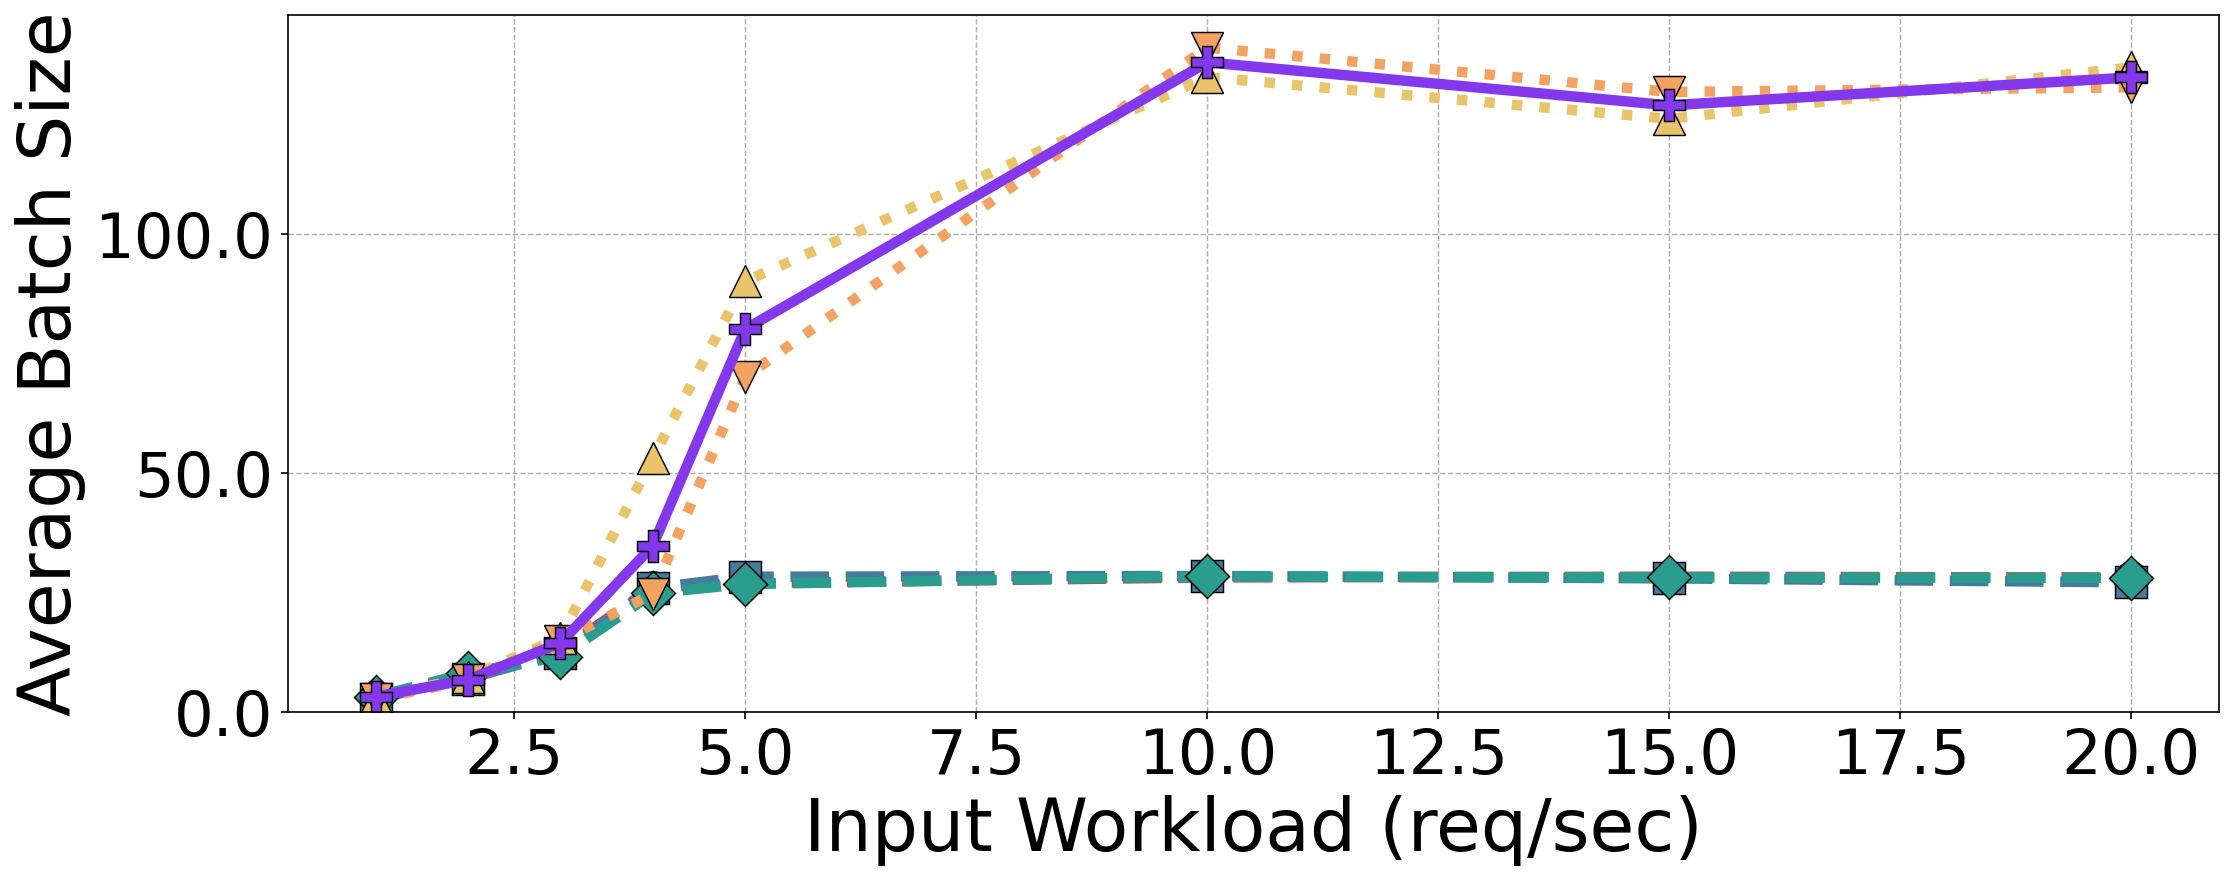
\includegraphics[width=\linewidth]{results/no_pref_sharing_plots/avg_batch_vs_rps.png}
\caption{Average Batch Size}
\label{fig:abs_no_pref}
\end{subfigure}
\hfill
\begin{subfigure}{0.30\linewidth}
    \centering
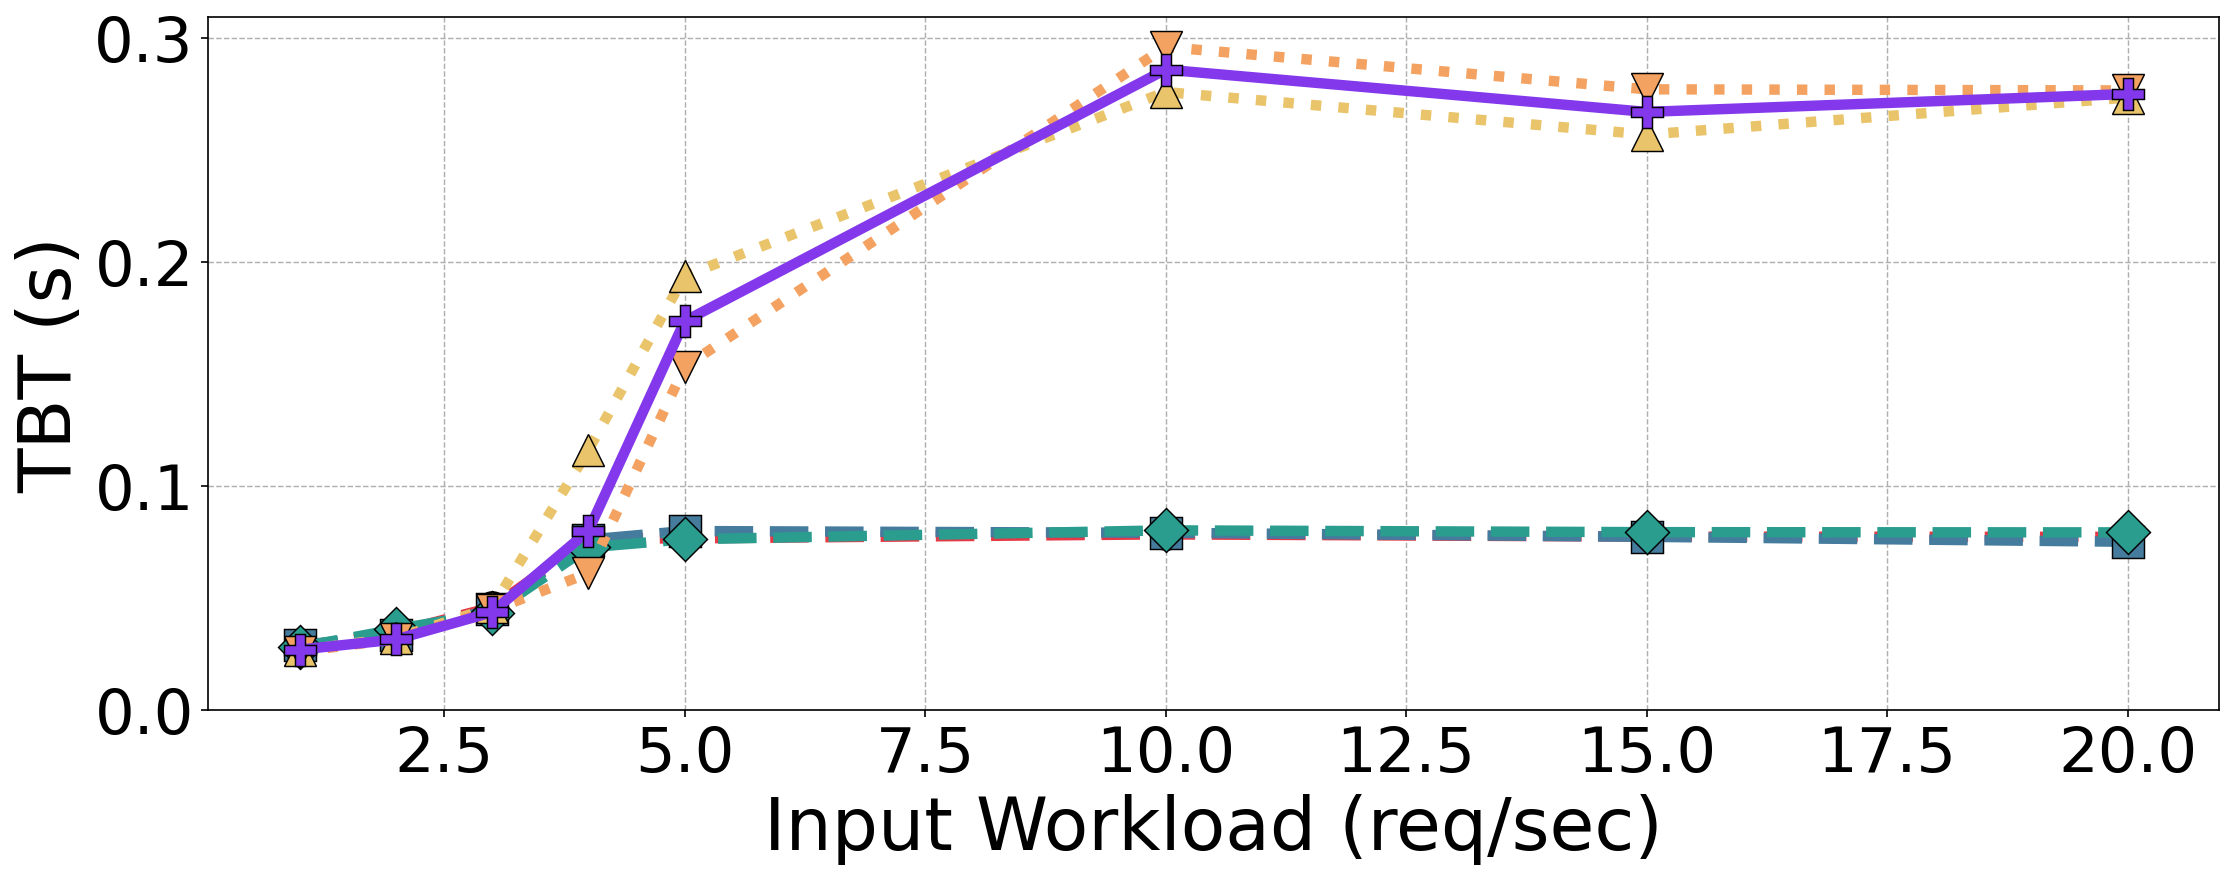
\includegraphics[width=\linewidth]{results/no_pref_sharing_plots/avg_timediff_vs_rps.png}
\caption{Time between tokens (TBT)}
\label{fig:tbt_no_pref}
\end{subfigure}
\caption{Workload with No Prefix Sharing}
\label{fig:no_pref}
\vspace{-10pt}
\end{figure*}

\subsection{Complexity Analysis of LPM and DFS-W}
\label{subsec:scheduling-complexity}
We provide a detailed complexity analysis of the two SGLang cache-aware scheduling policies discussed in \S\ref{sec:eval}: Longest Prefix Match (LPM) and Depth-First Search with Weighting (DFS-W). Let $W$ denote the number of requests in the waiting queue and $T$ the maximum prefix length. For each request, LPM performs prefix matching on the global radix tree, costing $\mathcal{O}(T)$ per request, and then sorts the queue by matched prefix length, adding $\mathcal{O}(W \log W)$. The total per-round cost is therefore $\mathcal{O}(W \cdot T + W \log W)$. The result is overhead that scales \textit{multiplicatively} with both queue size and context length. LPM implicitly acknowledges this by falling back to FCFS when $W > 128$ (which was disabled in our experiments). DFS-W avoids per-request traversal; instead, it performs a full traversal of the radix tree in each scheduling round. Let $B$ be the total number of radix tree nodes. DFS-W first propagates subtree request counts upward in $\mathcal{O}(B)$, then re-traverses in a depth-first manner, sorting children by weight at every level. The total cost is $\mathcal{O}(W + B \log B)$. The key problem is that $B$ reflects the server's accumulated history, not the current workload. The radix tree grows monotonically and is only pruned under memory pressure, so DFS-W's overhead increases over time, regardless of the current load. A server with a large accumulated cache ($B \gg W$) will incur high scheduling costs even during quiet periods. In summary, a burst of long-context requests penalizes LPM through the $W \cdot T$ term, while a large accumulated cache penalizes DFS-W through the $B \log B$ term. Either way, scheduling overhead can reach the same order of magnitude as GPU execution time. This demonstrates that identifying shared prefixes at runtime is fundamentally expensive and naive cache-aware scheduling can become the dominant bottleneck.

\subsection{Convergence of Bandit Policy}
\label{subsec:convergence_of_bandit_policy}
We also evaluate how quickly \Feather's bandit-based policy converges to a stable and efficient batching configuration. We construct a workload with five prefix groups, each containing 5K tokens, and issue requests at a rate of 5 per second. Figure~\ref{fig:convergence_of_bandit_policy} illustrates how the running batch size evolves over time for \Feather under its bandit-based policy. At the beginning, the system enters an exploration phase, during which \Feather experiments with different configurations and reaches relatively large batch sizes (around 500). However, these batches are heterogeneous. After this phase concludes (around 100 seconds), the system shifts to homogeneous batching, which yields higher throughput. As a result, \Feather converges to a significantly smaller batch size and maintains it for the remainder of the experiment.

\begin{figure}[t]
    \centering
    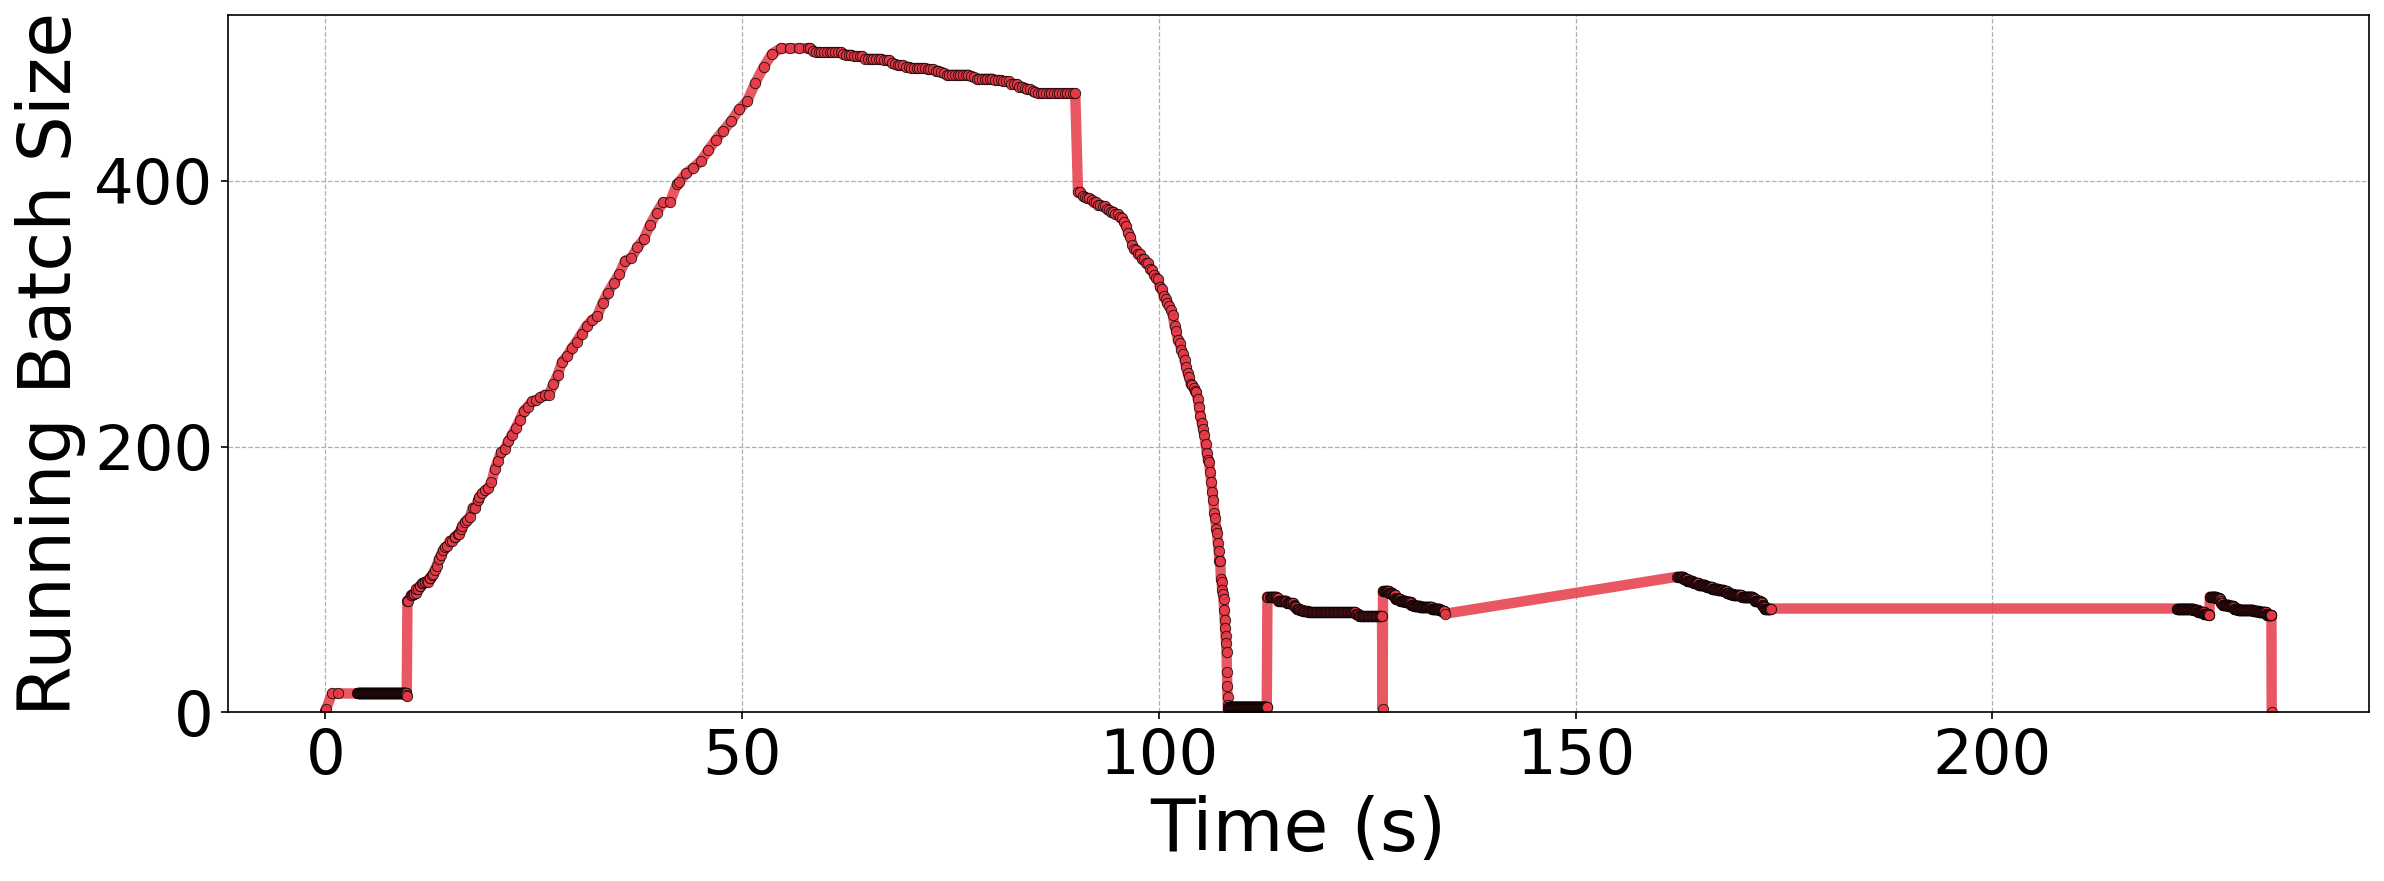
\includegraphics[width=0.8\linewidth]{results/rl_batch_size_plots/rl_policies_comparison.png}
    \caption{Convergence of Bandit Policy}
    \label{fig:convergence_of_bandit_policy}
    \vspace{-10pt}
\end{figure}

\subsection{RL Policy across Varying Workload}
\label{subsec:rl_policy_across_varying_worklaod}
We generate a workload consisting of five prefix groups, each containing 5K tokens. The input request rate varies over time—from 5 to 10 to 20 requests per second—and we measure the average batch size as a function of time for \Feather using its Bandit policy (Figure~\ref{fig:rl_policy_across_varying_worklaod}). From 0 to 200 seconds, the request rate is 5, and the batch size remains relatively low. Between 200 and 300 seconds, the rate increases to 10, leading to a noticeable rise in batch size. Finally, from 300 to 350 seconds, the request rate reaches 20, and the batch size peaks. (Fluctuations in the plot are due both to RL exploration and the workload being Poisson.) These results show that \Feather dynamically adapts the batch size in response to both prefix homogeneity (i.e., the number of requests sharing the same prefix group) and the current workload intensity.

\begin{figure}[t]
    \centering
    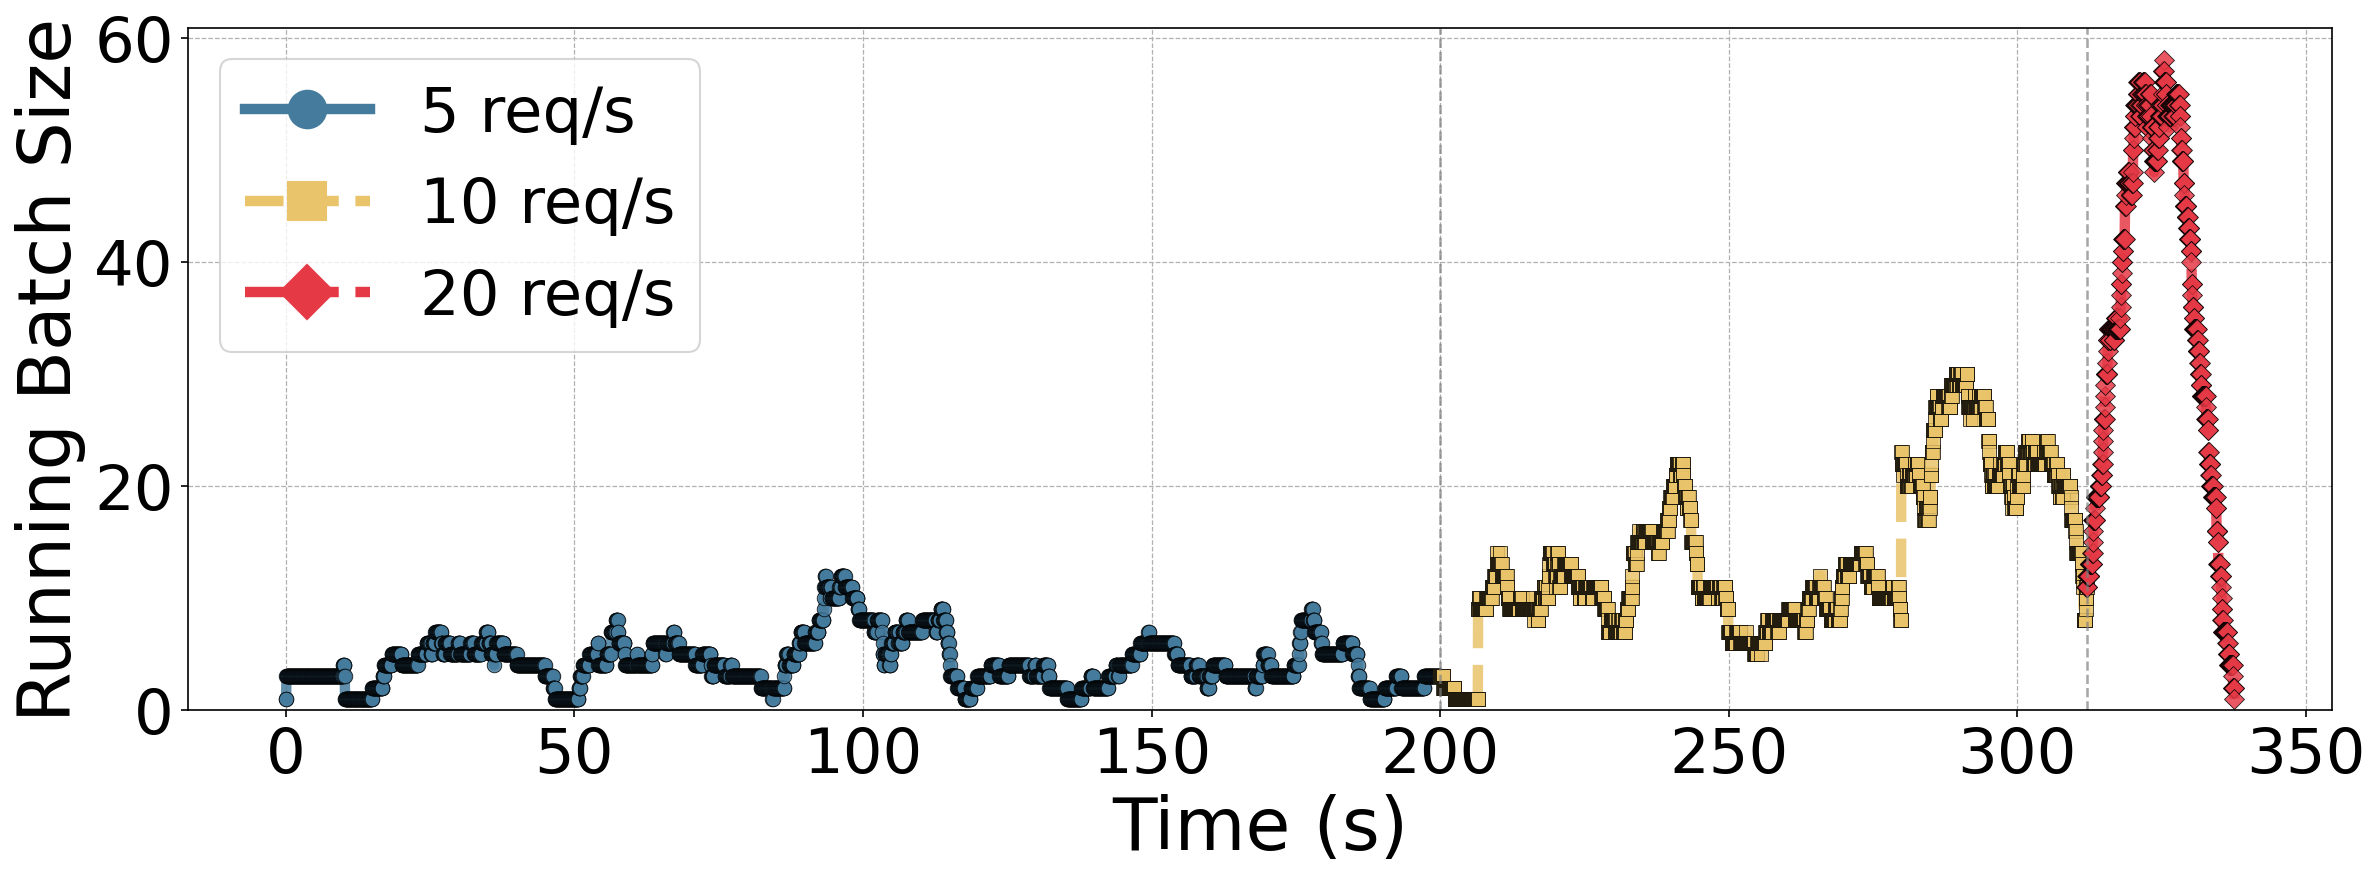
\includegraphics[width=0.8\linewidth]{results/rl_batch_size_plots/batch_size_over_time.png}
    \caption{Performance of Bandit across Varying Workload}
    \label{fig:rl_policy_across_varying_worklaod}
    \vspace{-10pt}
\end{figure}



\subsection{Workloads with No Prefix Sharing}
\label{subsec:workloads_with_no_prefix_sharing}
We next evaluate \Feather and compare it against other scheduling policies on a workload without prefix sharing; that is, no two requests share a common prefix. Figure~\ref{fig:no_pref} reports throughput, average batch size, and time between tokens (TBT) across a range of input rates. At higher input rates, vLLM-based policies begin to outperform SGLang policies, primarily due to their ability to form larger batches. Notably, even in the absence of prefix sharing, \Feather, powered by its adaptive RL-based policy—matches the performance of vLLM's FCFS scheduler. In contrast, SGLang policies achieve lower TBT, which can be attributed to their smaller batch sizes.

\subsection{Tensor Core Utilization across Policies}
\label{subsec:tensor_core_utilization_policies}
Figure~\ref{fig:req_per_sec_tenso_batch} compares tensor core utilization and average batch size across different request rates and scheduling policies. \Feather shows slightly lower utilization at low request rates due to forming smaller batches, but it still delivers higher throughput at these points (as seen earlier in Figure~\ref{fig:tp_vs_rps_l_5000_fam_5}). As the workload increases, \Feather gradually builds larger batches from prefix-homogeneous requests, and its utilization rises to match vLLM's FCFS. In contrast, SGLang's FCFS maintains relatively low utilization because it operates with consistently small batch sizes. Interestingly, even though SGLang's DFS-W and LPM achieve larger batch sizes, their utilization remains low. This is mainly due to CPU-side stalls between GPU executions, during which the GPU stays idle, effectively reducing overall utilization.


\begin{figure}[t]
\captionsetup[subfigure]{labelformat=simple}
    \renewcommand\thesubfigure{(\alph{subfigure})}
\centering
\begin{subfigure}{0.49\columnwidth}
    \centering
    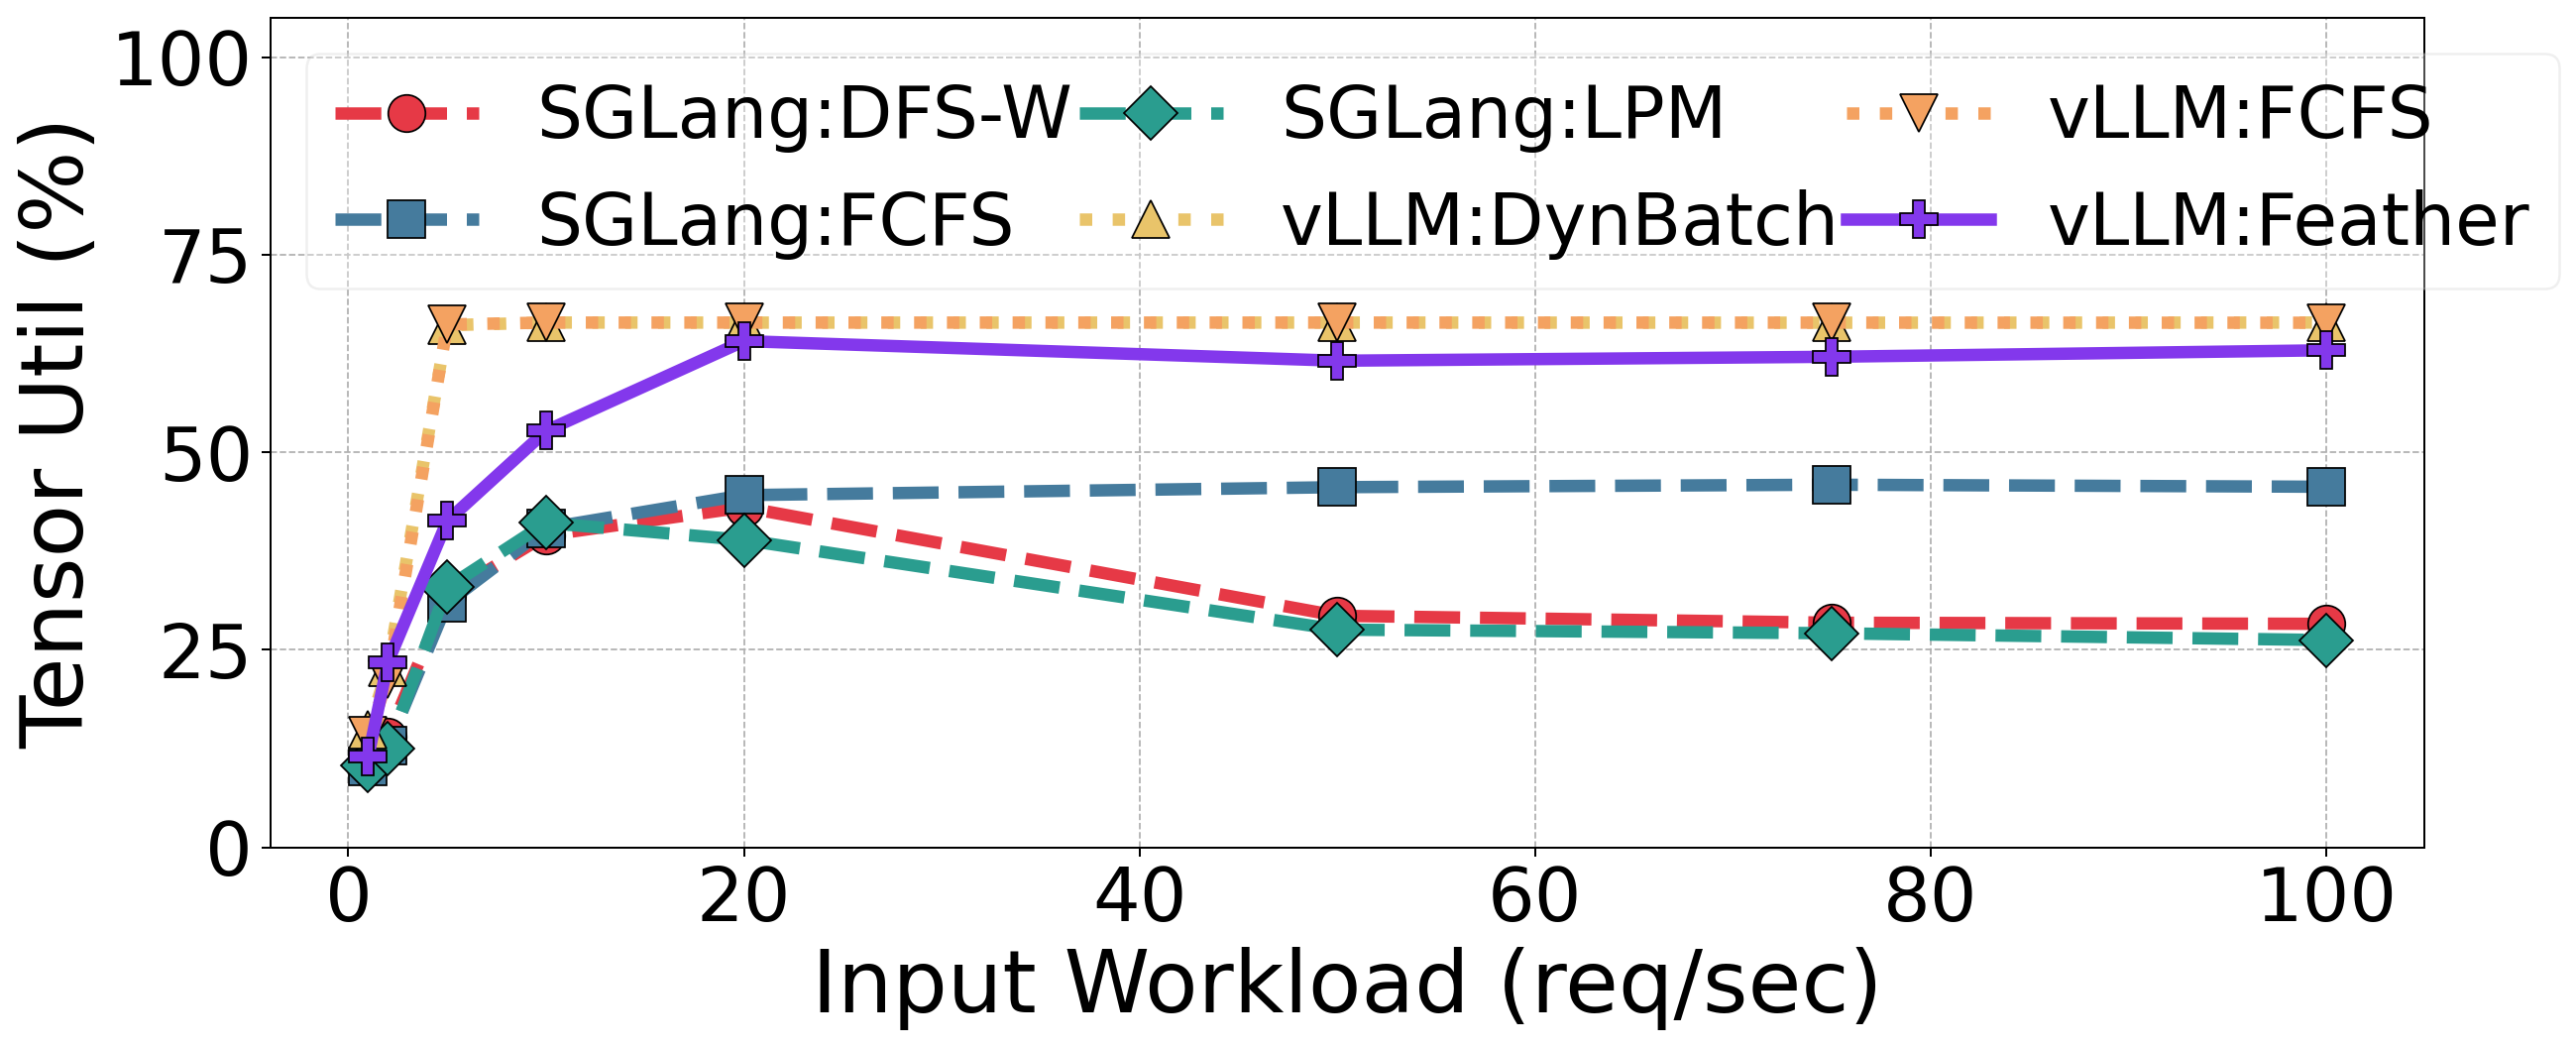
\includegraphics[width=\linewidth]{results/tenso_policy_plots/plot_tenso_vs_rps_policies.png}
    \caption{Tensor Core Utilization}
    \label{fig:tensor_core_utilzation_across_policies}
\end{subfigure}
\hfill
\begin{subfigure}{0.49\columnwidth}
    \centering
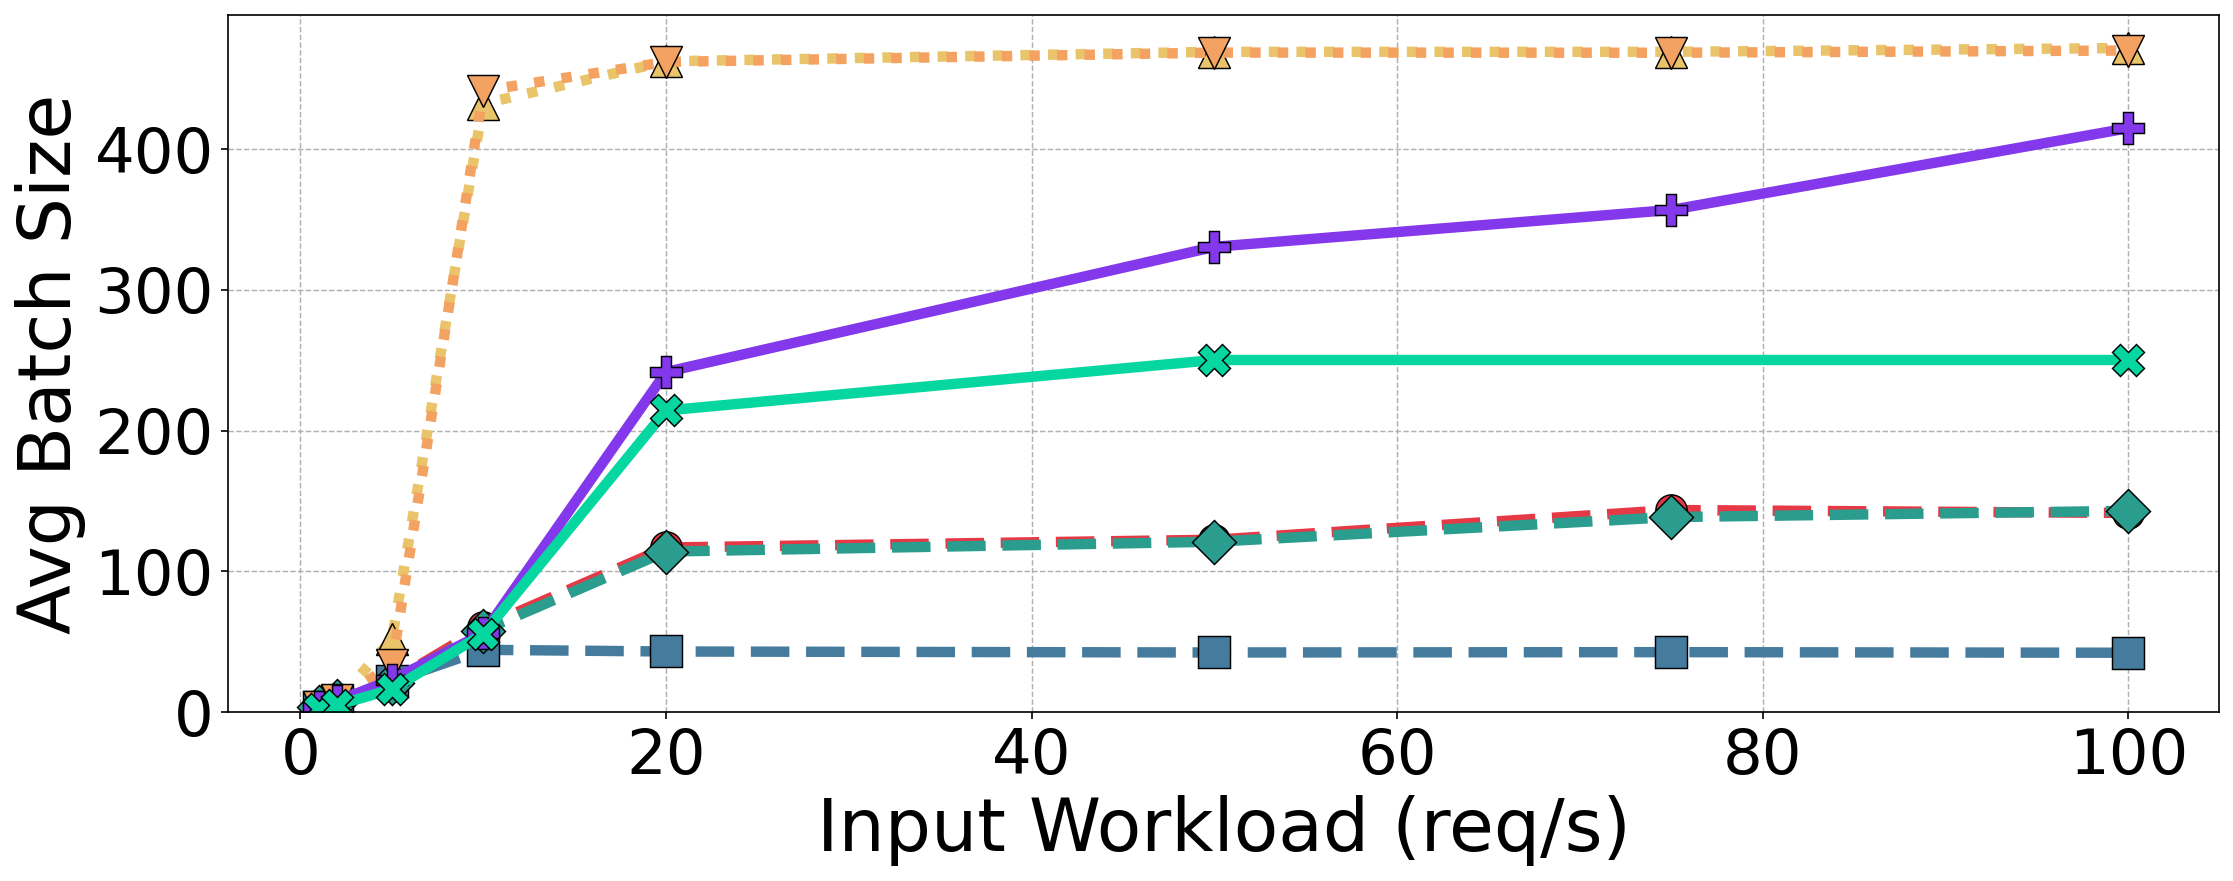
\includegraphics[width=\linewidth]{results/req_per_sec_plots/avg_batch_vs_rps.png}
\caption{Average Batch Size}
\label{fig:batch_size_across_policies}
\end{subfigure}
\caption{Input Workload}
\label{fig:req_per_sec_tenso_batch}
\vspace{-10pt}
\end{figure}

\section{Why the name \Feather?}
\label{sec:about_feather}
\Feather is named after the structural pattern of prefix-homogeneous batches in our system: a shared prefix forms a central shaft, from which individual requests branch out as they diverge, much like the barbs of a \Feather. The metaphor captures both the visual structure of our batches and the functional benefit of keeping prefix sharing requests together for better performance.